
\chapter{基于多种类多声强的ABR刺激增强方法}
本章节主要介绍本文提出的基于多种类多声强的ABR刺激增强方法,首先评估了多种刺激优化和信号处理技术对提高ABR测量效率的影响。通过实验比较了宽带Chirp、窄带Chirp、交错频率序列和 MLS 等新型刺激方式,以及自适应滤波、多种类降噪和主成分分析等信号处理方法。研究结果表明,不同刺激方式和处理技术的效果显著依赖于刺激频率和强度水平。
最后总结出最优的刺激和强度方法。

\section{任务背景与问题分析}
ABR作为客观听力评估技术,在婴幼儿、睡眠或麻醉患者等无法配合行为测听的特殊人群中具有不可替代的临床价值。然而,传统ABR检测存在两大核心瓶颈,第一耗时长:单耳全频段阈值评估通常需30-60分钟,导致临床筛查效率低下;第二信噪比敏感:低强度刺激下神经响应信号微弱,易受环境噪声干扰。
本章节主要从以下四个方向进行分析:
改进刺激声以提高响应幅度:
优化刺激速率:
降低背景噪声影响的刺激/信号处理技术:
自动检测方法。


\textbf{任务描述:}
本章节的研究聚集于ABR数据的采集,分析和结论。使用Neuroscan设备获得的成年人的ABR数据。记录主要是四通道记录,电极配置如下:Cz-Inion、Cz-A1、T1-T2、T1-A1,接地电极位于额头上。向每位受试者呈现了一系列广泛的刺激和序列。刺激通过插入式耳机以单耳方式在低(40 dB SL)和高(75 dB SL)水平上呈现。

\section{改进刺激声以提高响应幅度}
\textbf{宽带Chirp:}
声音在耳蜗中传播时,从基底部传至顶端大约需要 5–10 毫秒。点击刺激(Click)的高频成分(>2000 Hz)在耳蜗的基底区域产生最大位移,而低频成分则约在 10 毫秒后在顶端产生最大位移。这种由于频率传播时延而造成的时序差异会导致神经响应的同步性下降。
Chirp 刺激通过补偿这种频率相关的传播时间,使不同频率的成分在耳蜗中几乎同时到达其对应部位,从而实现更有效的幅度叠加,进而产生更强的神经响应。
研究表明,宽带Chirp波形在几毫秒内频率逐渐上升,在大多数刺激强度(< 60 dB SL)下能够引发比点击刺激更大的 V 波幅度(Dau 等, 2000)\cite{dau2000optimized}
\begin{figure}[H]
  \centering
  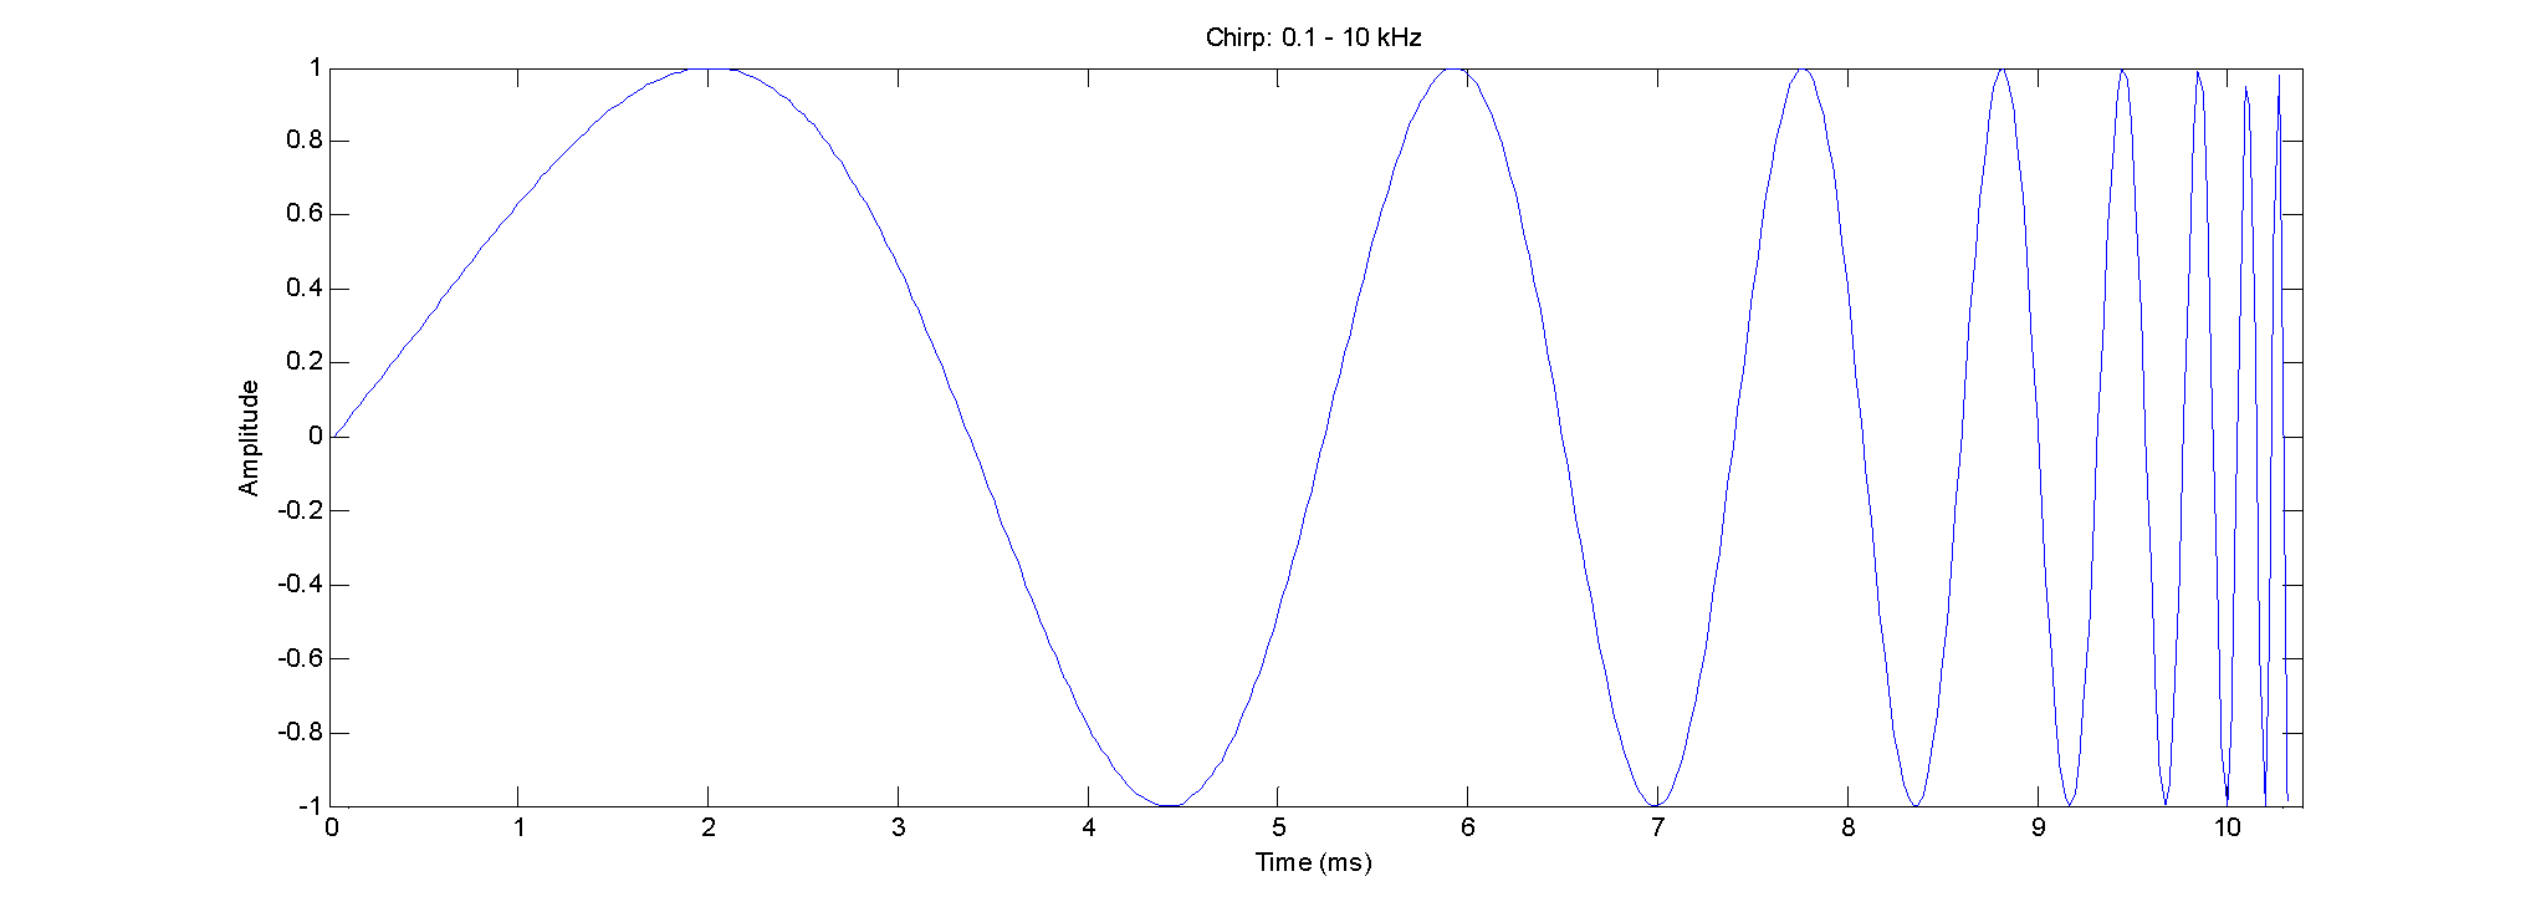
\includegraphics[width=1\textwidth]{images/Chirp.png}
  \caption{宽带Chirp信号(0.1 Hz 至 10 kHz)}
  \label{fig:ChirpfrequenceRange}
\end{figure}

\textbf{特定频率Chirp:}

除了用于全频段刺激的宽带 Chirp,本文也尝试使用频率有限的Chirp信号,称为频率特异性(Frequency-Specific)Chirps,来诱发ABR。Wegner 和 Dau(2002)发现,在低频(250 Hz)下,用一个以250 Hz为中心的 Chirp 刺激,比250 Hz的Tone刺激(Tone)产生更大的ABR响应幅度,尤其是在低到中等刺激强度下。
在本实验中使用的频率特异性 Chirp 波形具有以下特点:
频率范围约为一个倍频程(例如中心频率为500 Hz时,覆盖大约350-700 Hz);使用了高斯窗进行加窗,以控制其在时间域和频率域的形状。

\begin{figure}[H]
    \centering
    \begin{minipage}{0.48\textwidth}
        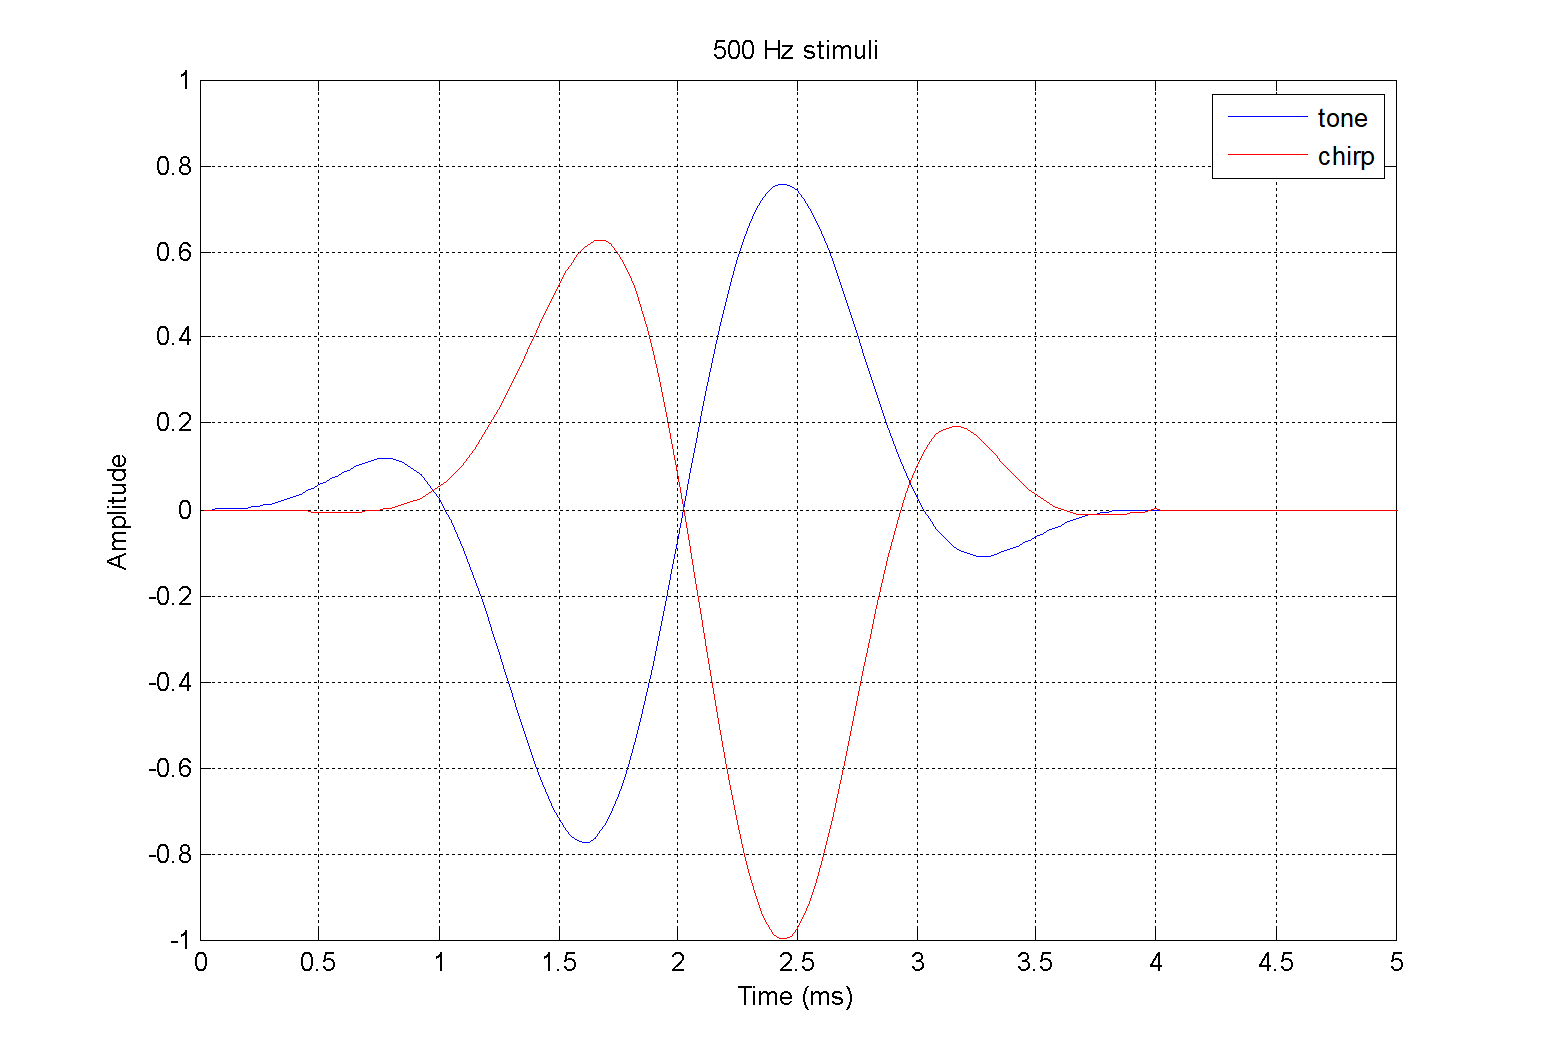
\includegraphics[width=\textwidth]{images/500hzStimuli.png}
    \end{minipage}
    \hfill
    \begin{minipage}{0.48\textwidth}
        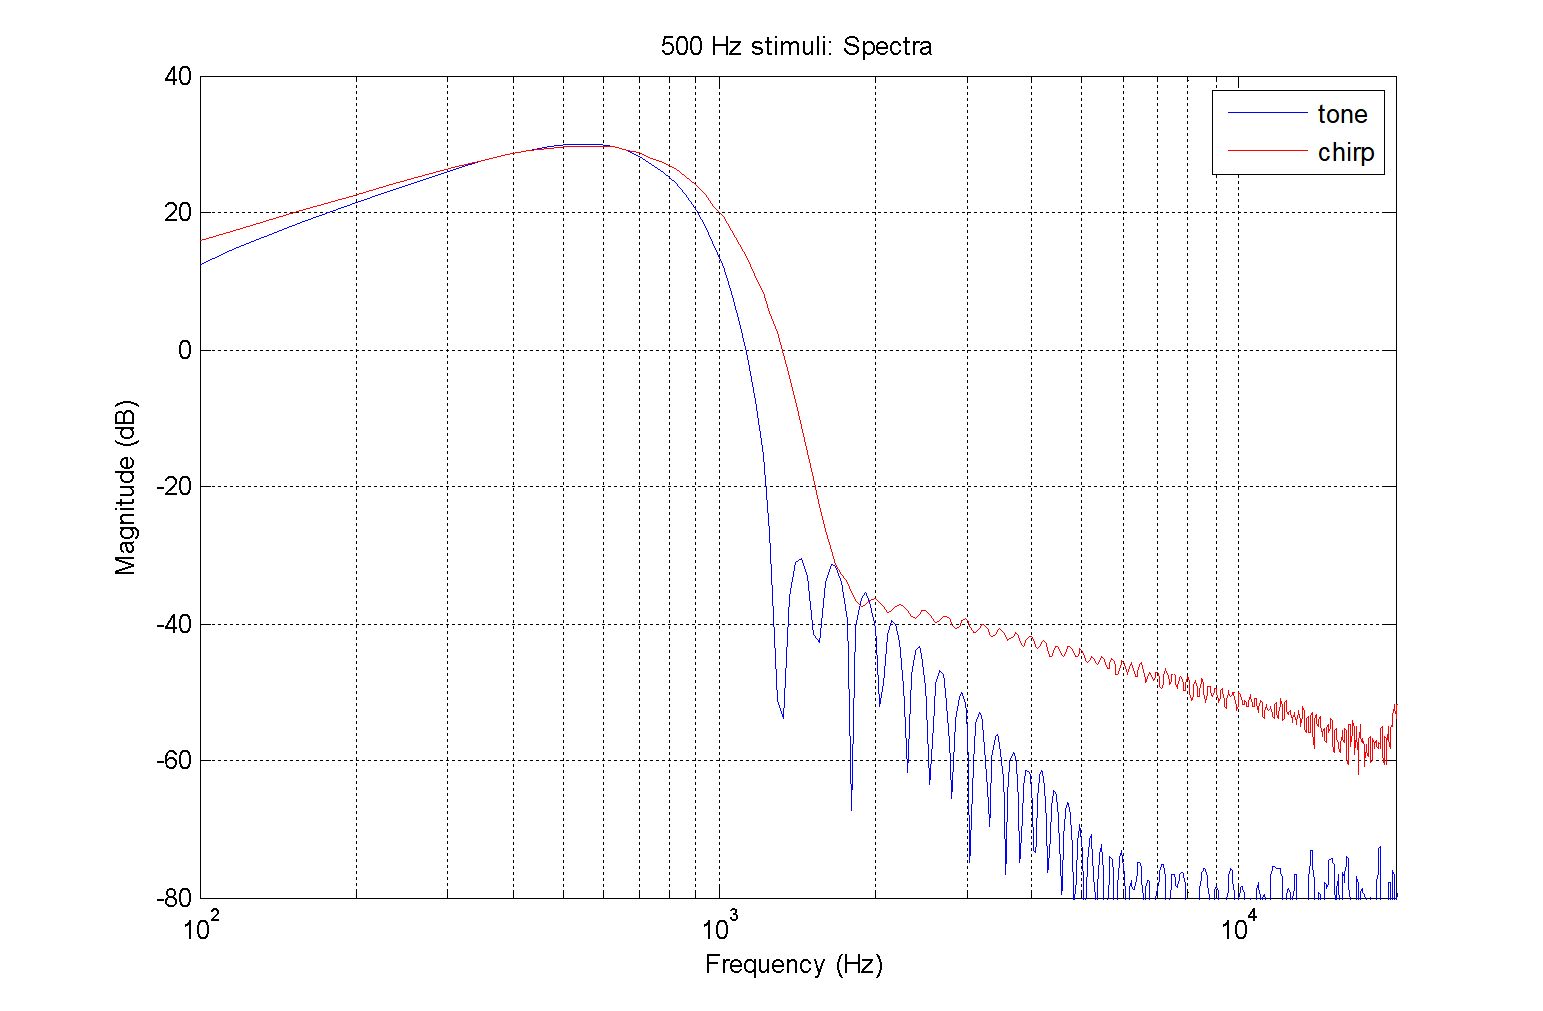
\includegraphics[width=\textwidth]{images/500hzSpectra.png}
    \end{minipage}
    
    \vspace{0.2cm}
    
    \begin{minipage}{0.48\textwidth}
        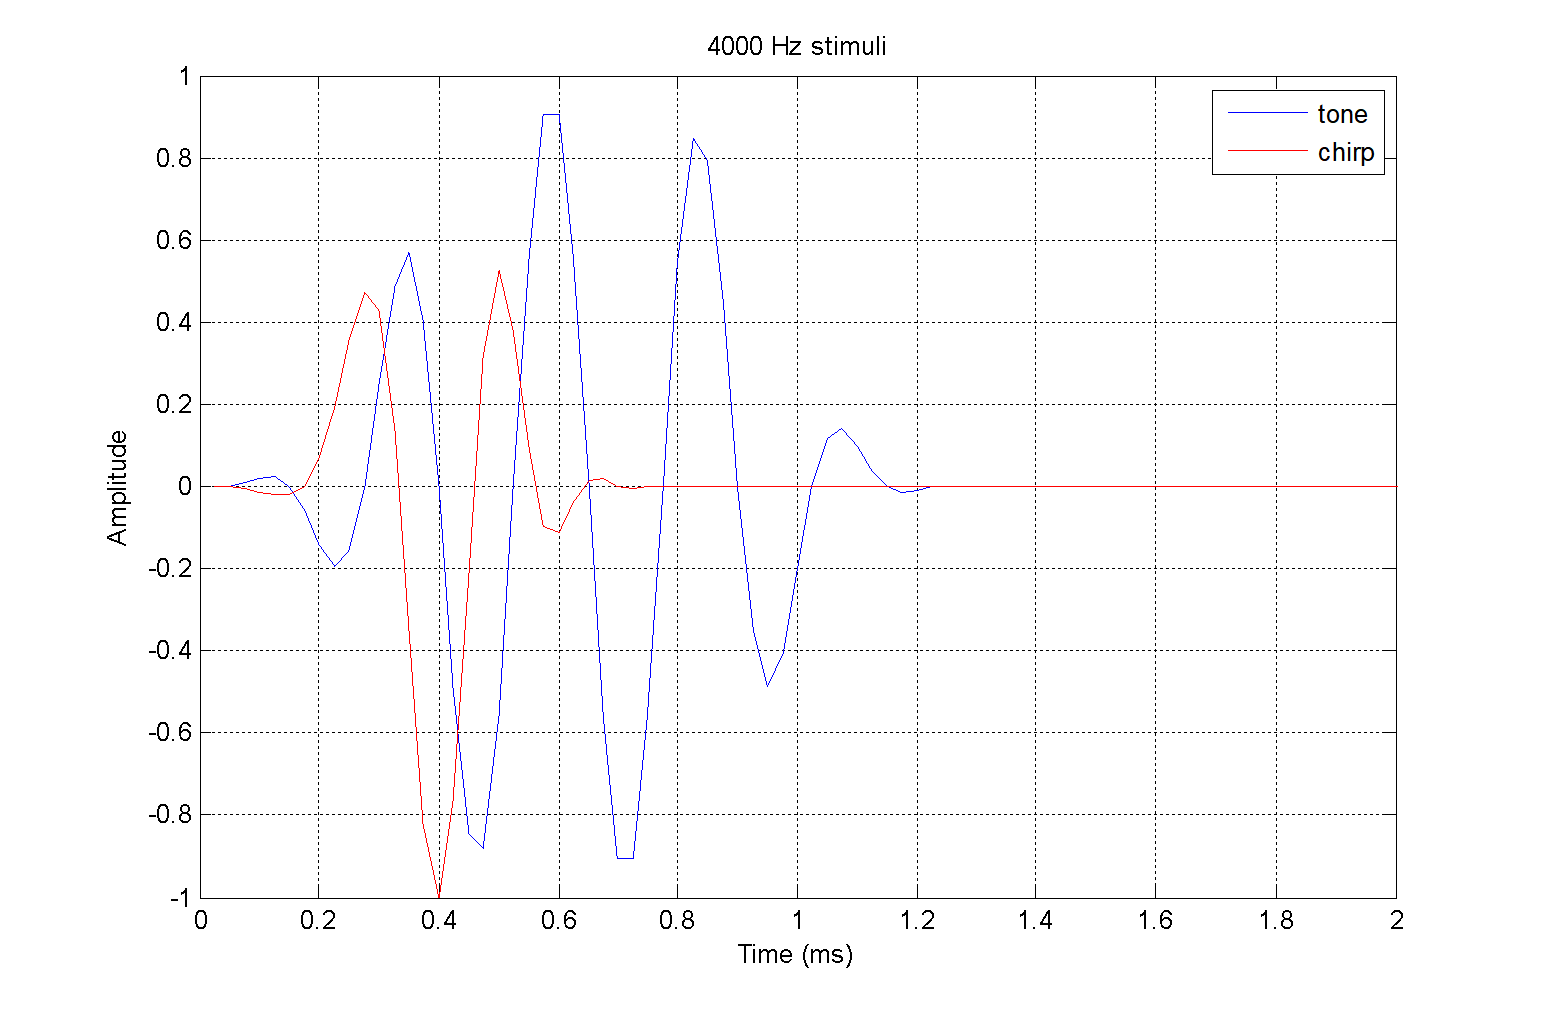
\includegraphics[width=\textwidth]{images/4000hzStimuli.png}
    \end{minipage}
    \hfill
    \begin{minipage}{0.48\textwidth}
        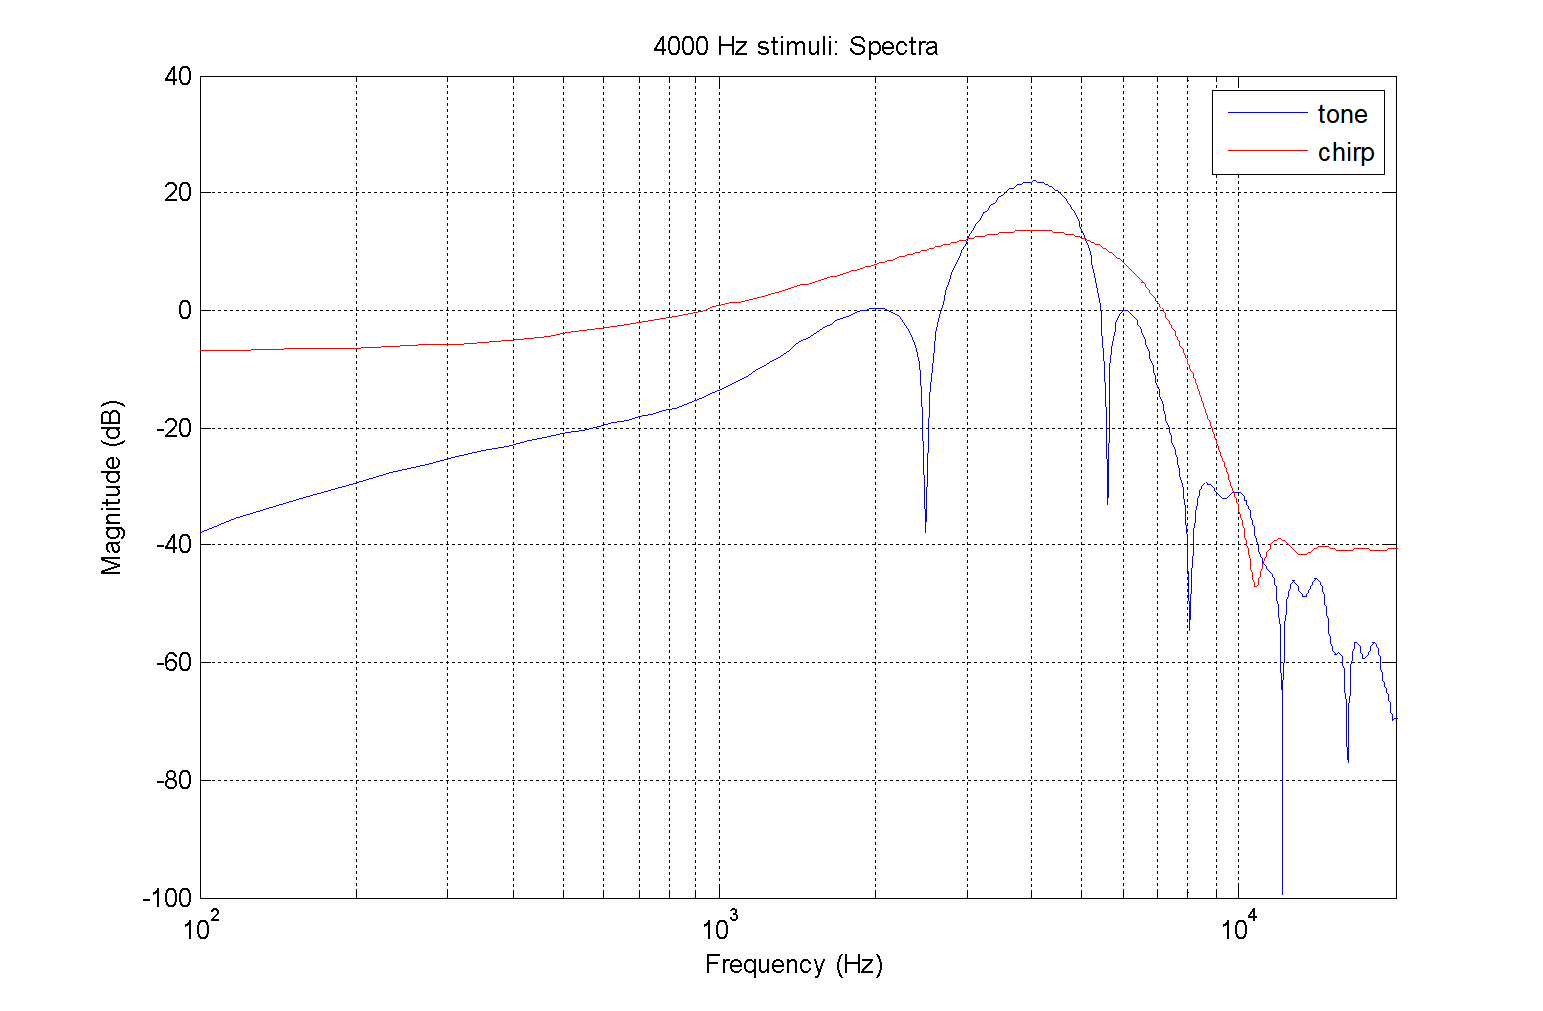
\includegraphics[width=\textwidth]{images/4000hzSpectra.png}
    \end{minipage}
    \caption{4 kHz、500 Hz的Tone和窄带Chirp刺激的时域波形与频谱图}
    \label{fig:4k500hzToneAndNarrowbandChirp}
\end{figure}
\FloatBarrier 
\section{优化刺激速率}

\textbf{交错频率:}
本研究精选了四个具有代表性的测试频率:4000Hz、2000Hz、1000Hz和500Hz。这些频率的选择基于以下考虑:

1)覆盖人类语音感知的关键频率范围;

2)代表耳蜗基底膜不同区域的特征响应; 

3)临床听力评估的标准测试频率点。

本设计的4频率设置既保证了足够的频率覆盖,又避免了过多频率导致的信号干扰问题。刺激间隔为18毫秒,音列之间的暂停时间为50毫秒。在无掩蔽噪声的条件下,交错频率序列中使用的单个Tone与单频刺激(每秒20个音爆)中使用的Tone完全一致。

\begin{figure}[H]
  \centering
  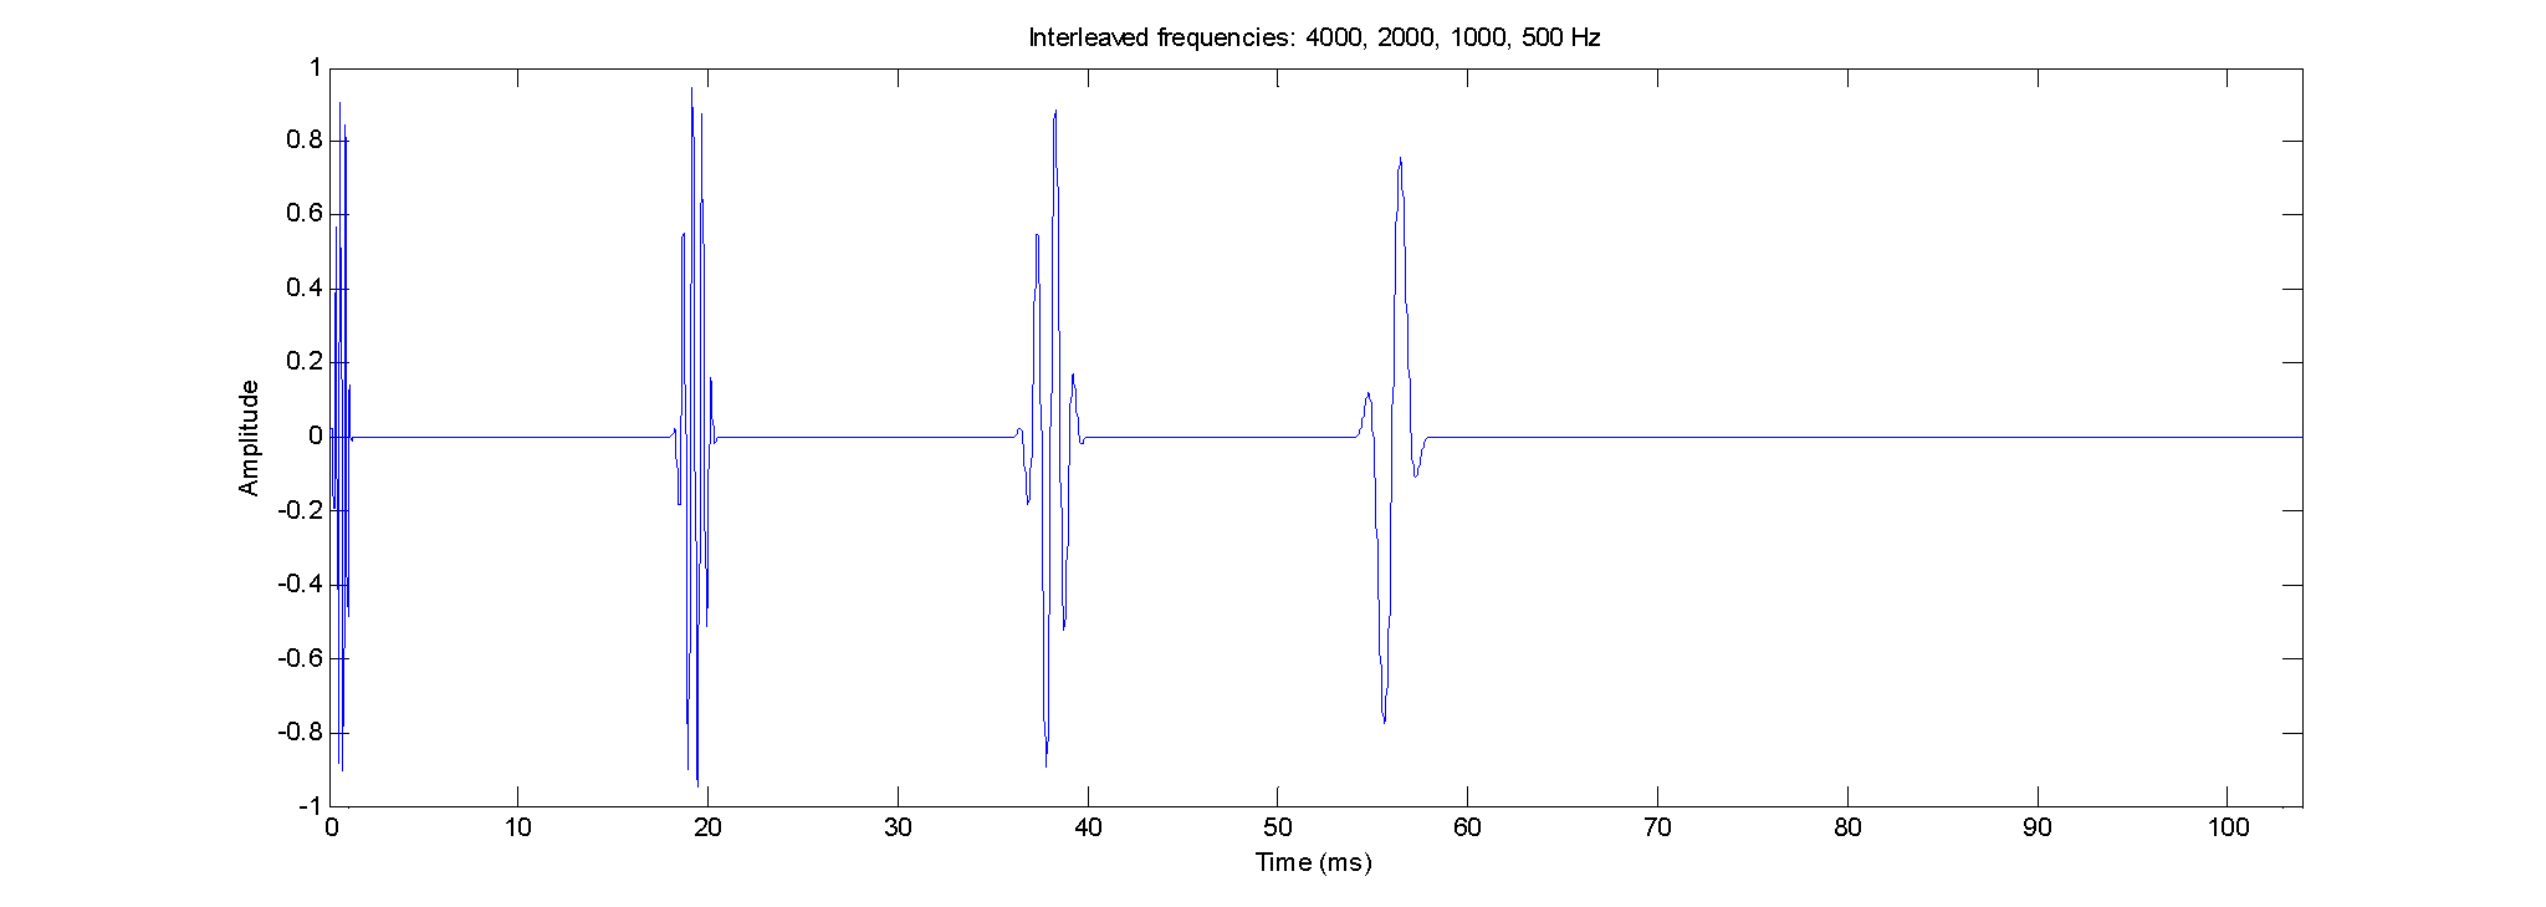
\includegraphics[width=1\textwidth]{images/InterleavedFrequencies.png}
  \caption{交错频率Tone的刺激序列}
  \label{fig:InterleavedFrequencies}
\end{figure}

\textbf{最大长度序列}

在传统刺激方式中,为避免响应之间的重叠,刺激速率通常受到神经反应持续时间的限制。使用最大长度序列(Maximum Length Sequence, MLS)可以显著提高刺激速率。MLS 是一种伪随机二进制序列,具有以下特殊自相关性质:其自相关函数在延迟为 0 时为序列长度 L,在其他任意延迟处均为 -1。这一特性使得即便多个刺激引发的神经反应重叠,仍可以通过反卷积将其有效分离。

在一个长度为 $L = 2^N - 1$ 的刺激序列中(其中 $N$ 为序列的阶数),共有 $2^N - 1$ 个点击声(Clicks)和 $2^N - 2$ 个静音间隔。该序列中有一半的脉冲之间的间隔为最小刺激间隔(Interstimulus Interval, ISI),其余的脉冲则以ISI的整数倍间隔分布。序列越长,ISI的变化也越大。

标准的 MLS 去卷积方法假设序列中所有刺激所诱发的反应是恒定的,然而实际上神经反应在高刺激速率下会发生适应性变化。具体而言:

\begin{enumerate}
    \item 随着刺激速率的增加,波形峰的潜伏期(Latency)会延长;而刺激强度越高,潜伏期越短;
    \item 随着刺激速率的增加,波形峰的幅度(Amplitude)会减小;而刺激强度越高,幅度会增加。
\end{enumerate}

由于不同ISI引起的反应幅度和潜伏期的变化,会导致在MLS反应的去卷积结果中出现未被抵消的波峰,从而增加了额外噪声。因此,在进行去卷积时,需要采用更复杂的非线性处理方法来解决这一问题。

\vspace{0.5em}
\noindent 其他需要考虑的因素包括:

\begin{itemize}
    \item \textbf{序列长度:} 序列过短时更容易被识别,也会在单位时间内重复出现更多次。若受试者能识别MLS序列的节奏,可能引发除单个刺激响应外的其他脑电反应。然而,序列越长,其ISI变化越大,反应波形的变异性也随之增加。本研究 ABR 试验中选择的序列长度为63(即MLS阶数为6)。
    
    \item \textbf{MLS速率:} 最优的MLS刺激速率(即在固定测试时间下获得最佳信噪比)与刺激强度有关。若仅考虑波V的检测,200~Hz 是超阈值条件下的最佳速率,而接近阈值时则以300~Hz表现最佳。本研究采用的刺激速率为250~Hz。
\end{itemize}

虽然MLS最常与Clicks一起使用,但也有研究探索了与Tone-Burst刺激及带限Chirp刺激的结合。

本研究中使用了中心频率为4~kHz和500~Hz的Tone-Burst刺激,以及以4~kHz和500~Hz为中心频率的窄带Chirp刺激。所用刺激序列的时域波形如图~\ref{fig:4k500hzToneAndNarrowbandChirp} 所示。

\begin{figure}[H]
    \centering
    \begin{minipage}{0.48\textwidth}
        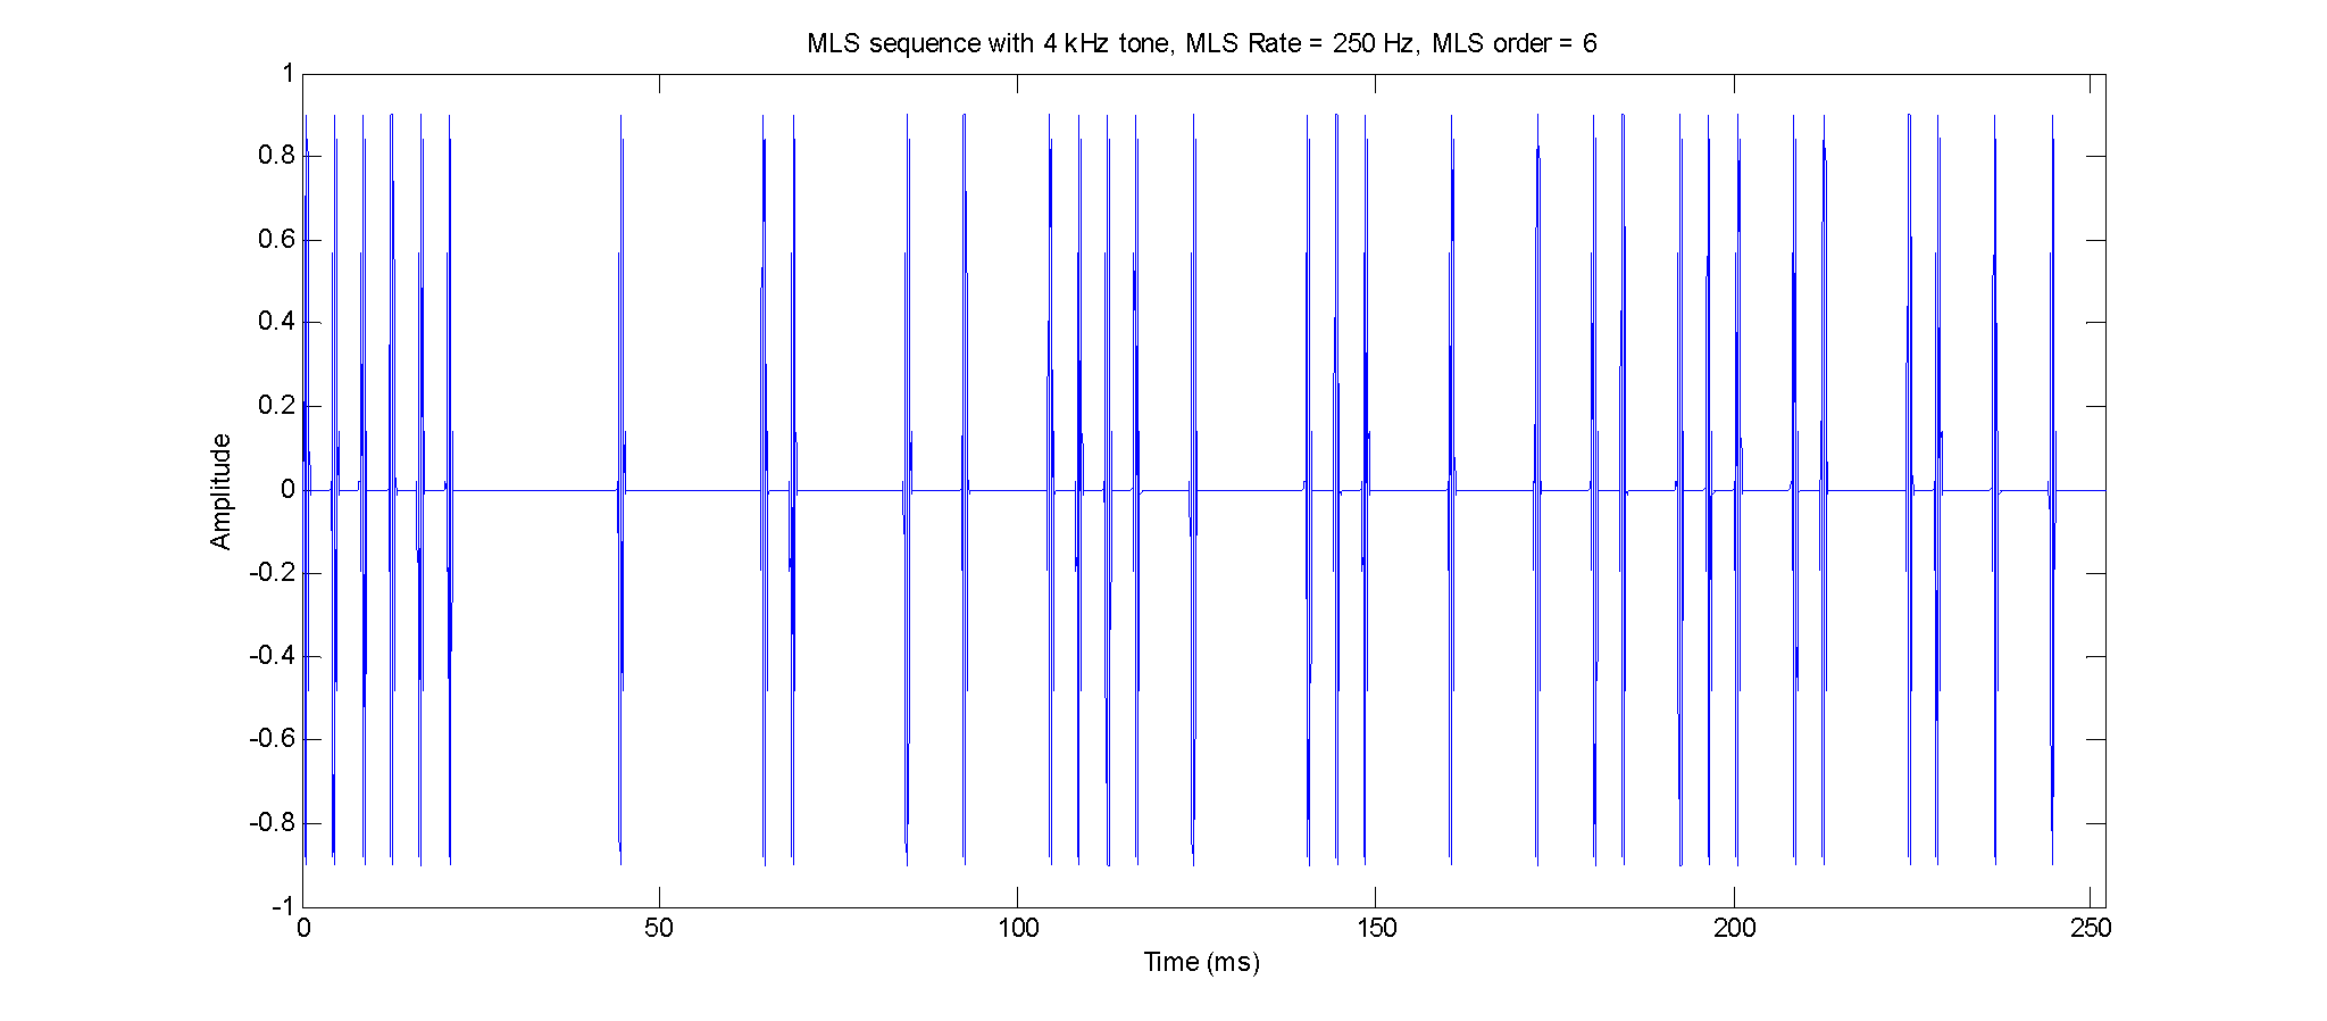
\includegraphics[width=\textwidth]{images/msl_sequence_with4kHztone.png}
    \end{minipage}
    \hfill
    \begin{minipage}{0.48\textwidth}
        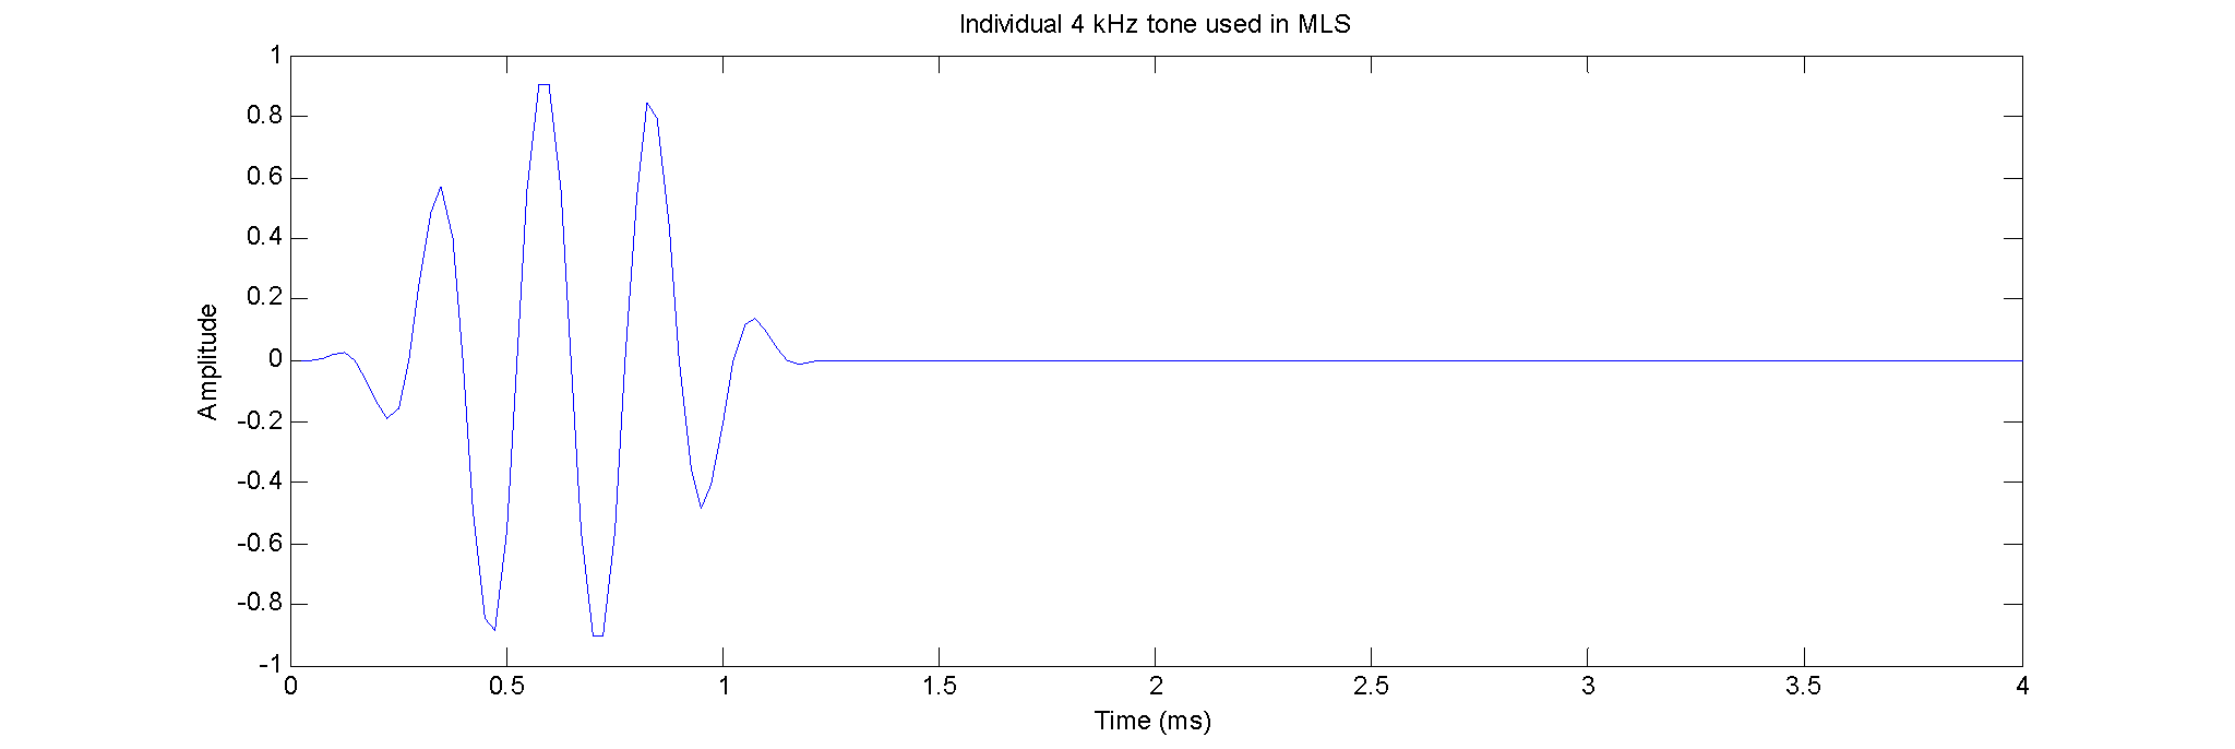
\includegraphics[width=\textwidth]{images/individual4kHzToneInMLS.png}
    \end{minipage}
    
    \vspace{0.2cm}
    
    \begin{minipage}{0.48\textwidth}
        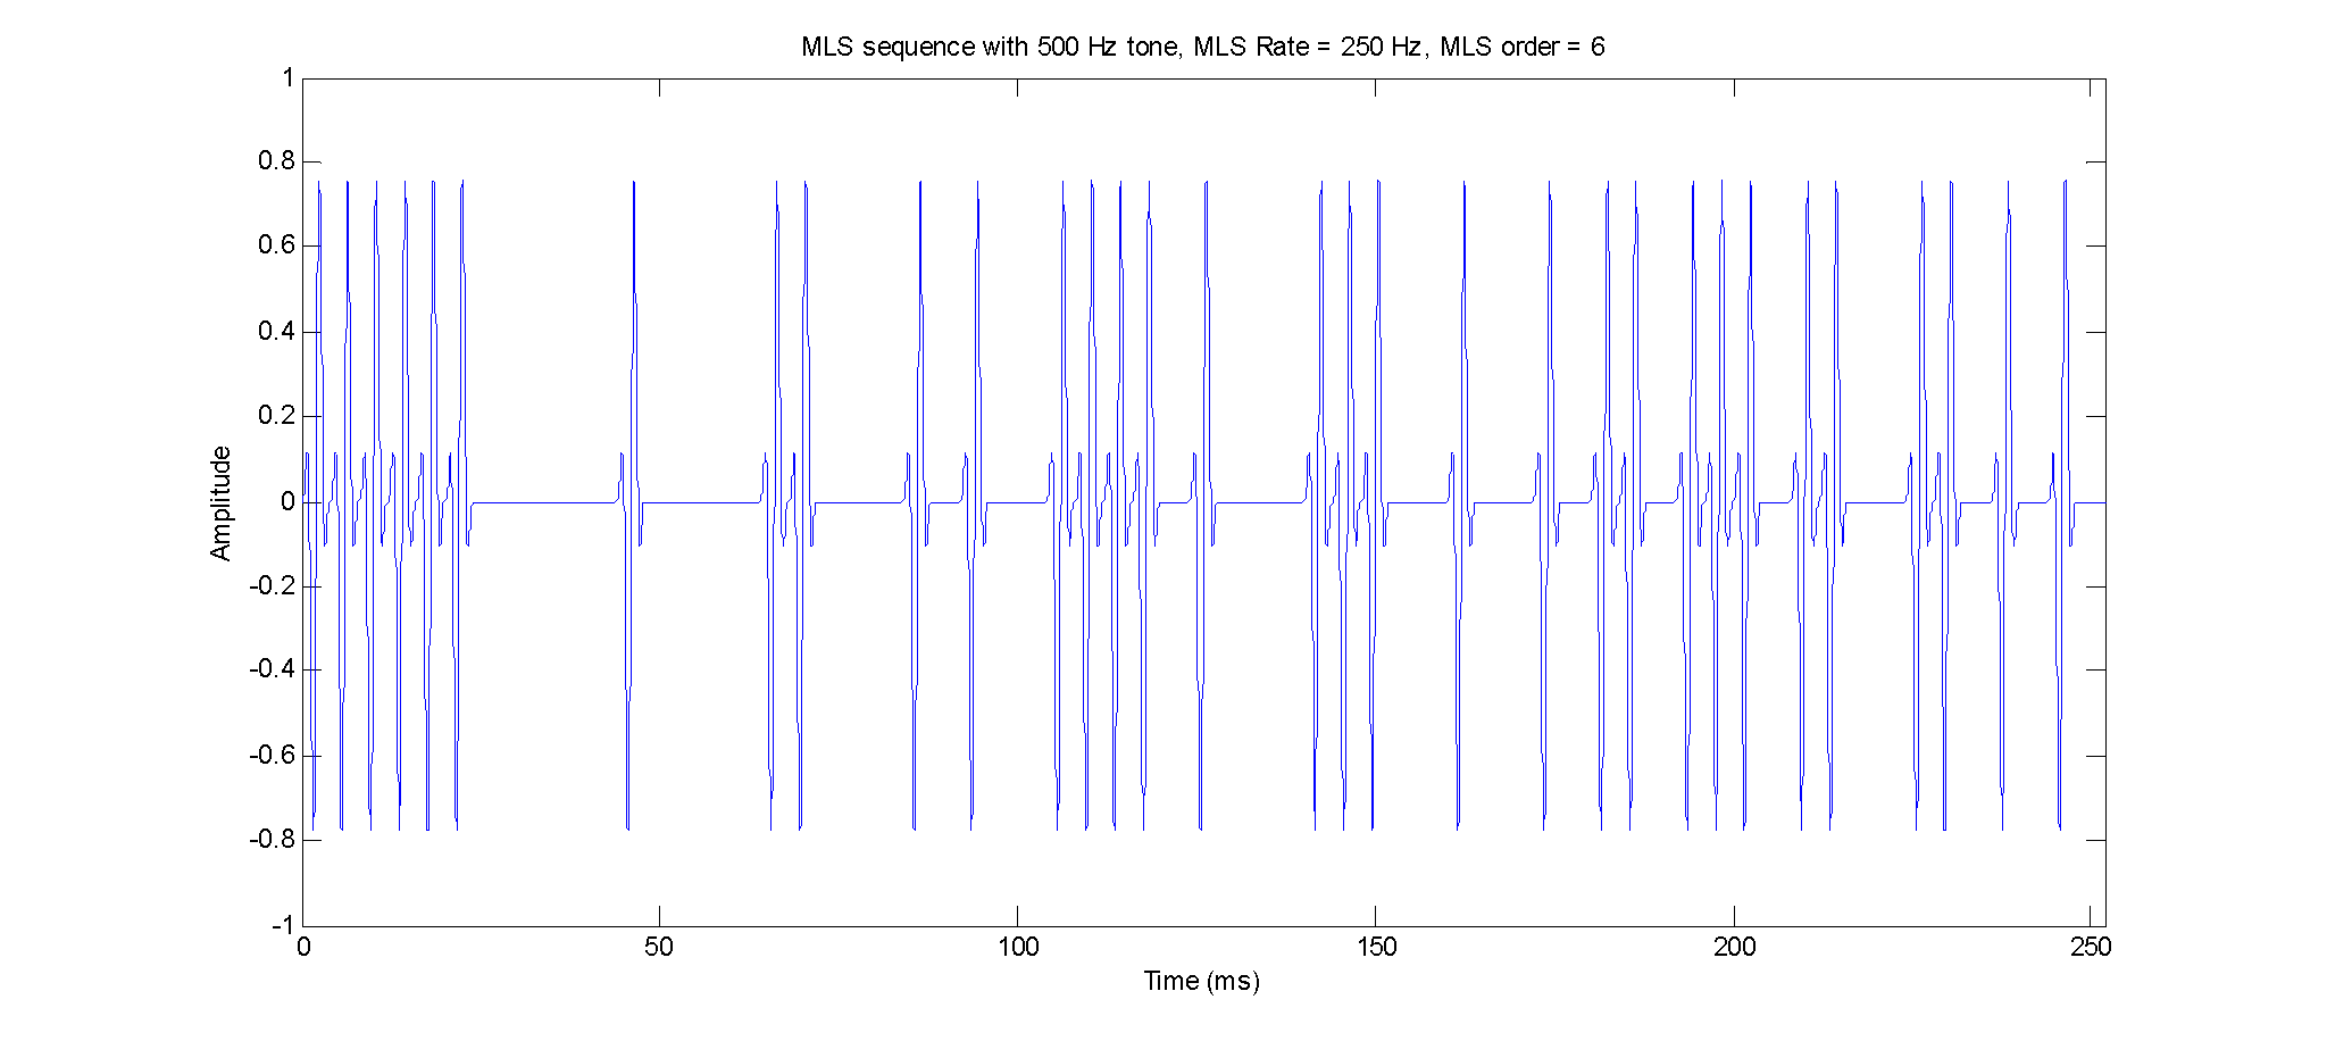
\includegraphics[width=\textwidth]{images/msl_sequence_with500Hztone.png}
    \end{minipage}
    \hfill
    \begin{minipage}{0.48\textwidth}
        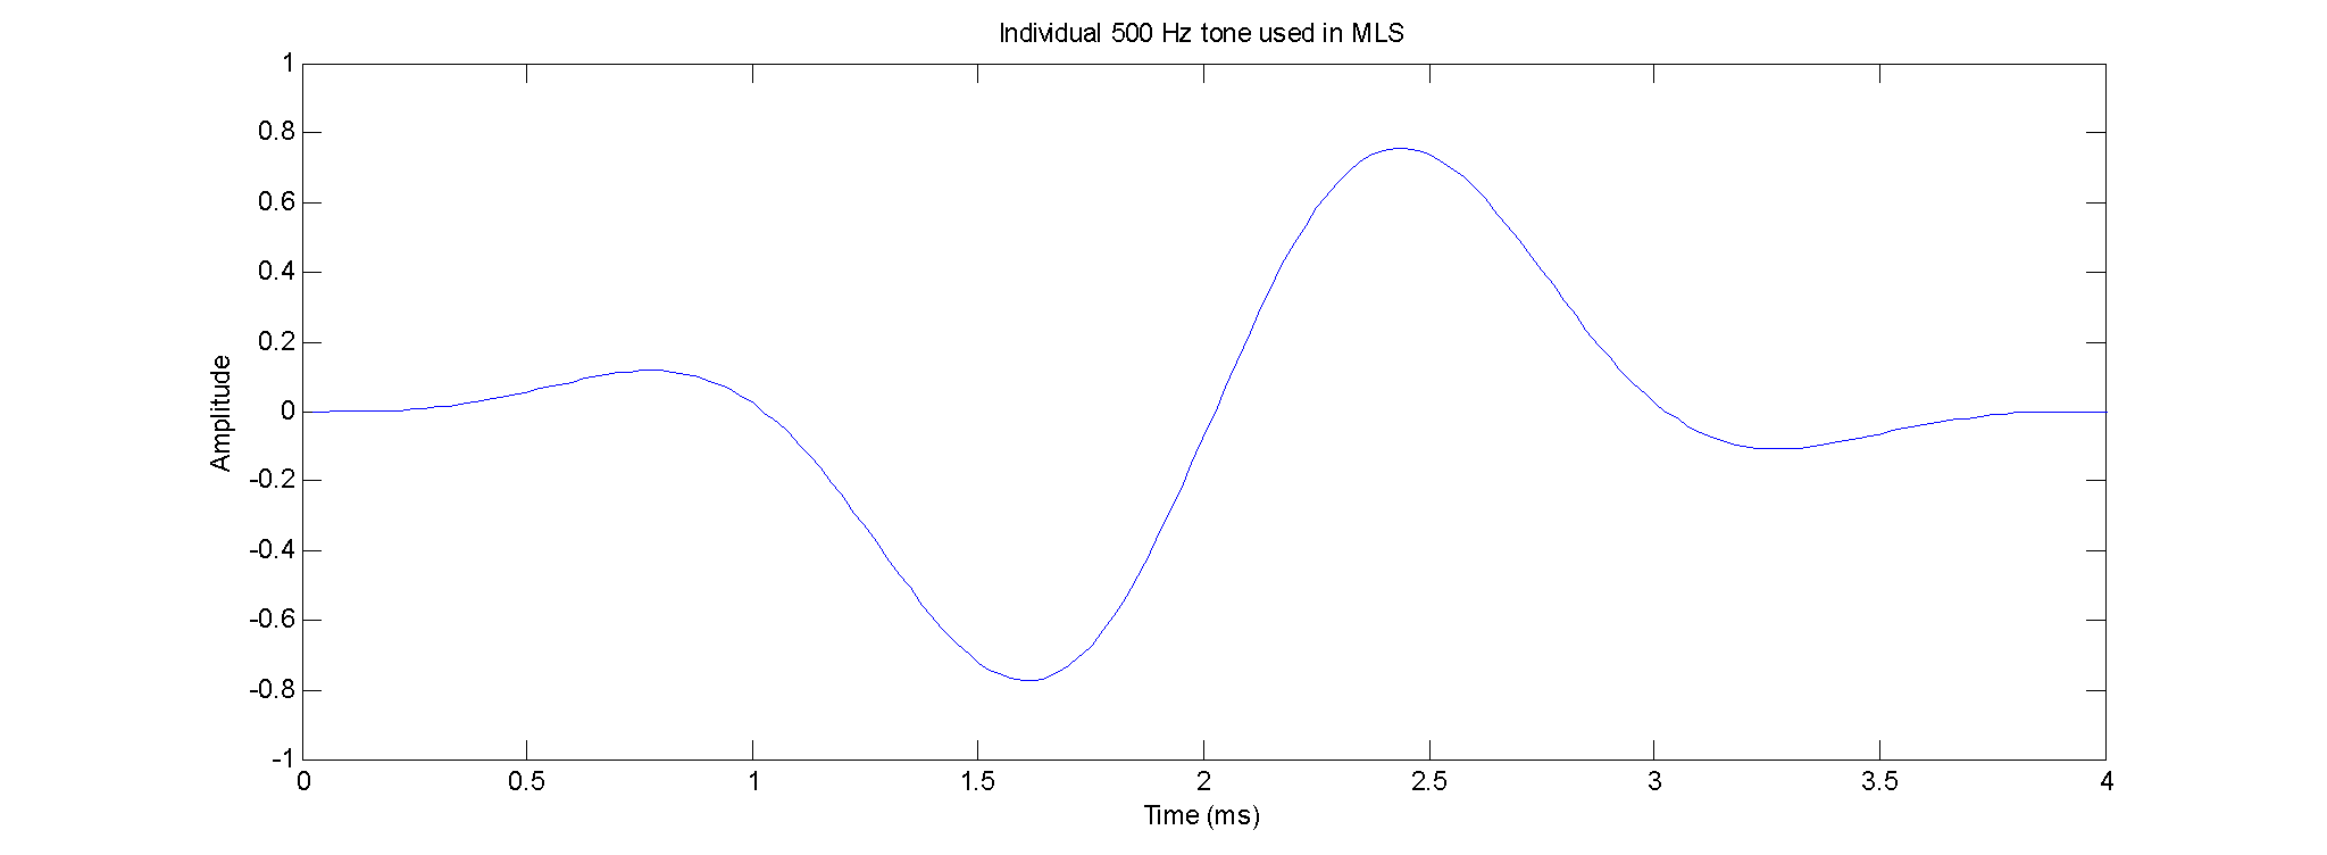
\includegraphics[width=\textwidth]{images/individual500HzToneInMLS.png}
    \end{minipage}
    \caption{4kHz、500HzTone的时域波形与频谱(MLS序列)}
    \label{fig:4k500hzToneAndNarrowbandChirp}
\end{figure}

\noindent \textbf{注意:}在500~Hz刺激中,采用了缩短的波形形式,以避免高频率刺激序列中出现的刺激重叠。这一配置不同于常规刺激中常用的2-0-2或2-1-2周期结构。


\section{改进的刺激与处理方法以降低噪声影响}
\subsection*{平均技术}

本研究中所有测试记录均应用了以下三种平均方法:
\paragraph*{普通平均}
时域集合平均(Time-domain ensemble averaging)是提高 SNR 最常见且基本的方法。假设 ABR 信号保持恒定且噪声为平稳噪声,平均 N 次后噪声贡献将按 $1/\sqrt{N}$ 的比例减小。在平均之前先进行滤波,以去除信号能量较少频段的背景噪声。本研究中使用的带通滤波器通带范围为 100–3000 Hz。
\[
\overline{X} = \frac{1}{N} \sum_{i=1}^{N} X_i
\]
\paragraph*{加权平均}
通常,背景噪声在整个记录过程中不会保持平稳,某些单次噪声爆发可能会显著影响平均结果的 SNR。对传统平均的一种改进是为每个扫掠分配一个基于该扫掠内噪声方差的权重因子,噪声越大的扫掠权重越低。其加权平均公式为:
\begin{align}
\overline{X_w} &= \frac{1}{C_N} \sum_{i=1}^N \frac{X_i}{V_i} \\
C_N &= \sum_{i=1}^N \frac{1}{V_i} \quad \text{(其中 } V_i \approx \frac{1}{N}\sum X_i^2 \text{)}
\end{align}

\paragraph*{区块加权平均}
该方法与加权平均类似,不同之处在于使用扫掠区块估计噪声方差。区块大小可为 10 至 250 次扫掠,较小区块尺寸更容易获取低噪声扫掠。这种方法也被称为贝叶斯加权。

加权平均优于伪迹拒绝(Artifact Rejection),因为它降低了噪声扫掠的影响,而无需事先设定拒绝阈值。

\subsection*{多通道噪声抑制}

多通道噪声抑制技术引入了额外电极,用于检测与主电极记录电压中噪声相关的信号。通过回归分析,计算两个通道之间的关系,从主通道信号中减去一个比例缩放后的辅助通道信号,从而获得降噪后的信号。

为了达到最佳效果,应将电极布置为:主通道信号强,辅助通道信号弱但与主通道噪声高度相关。与皮层反应不同,ABR 的 V 波在头皮多个区域都很强,尤其在对侧(Cz–A2)和水平阵列(A1–A2)上。

以下电极布置用于本研究:Cz – Inion、 Cz – Inion、 Cz – A1、  T1 – T2、 T1 – A1。
少数受试者也使用以下布置:Cz–A2、A1–A2、Shoulder–Inion。

\textbf{注意事项:}
\begin{itemize}
    \item Cz–Inion 相比 Cz–A1 记录到更大波幅的 V 波,但背景噪声也更高。
    \item T1–A1 的反应与 Cz–A1 类似。
    \item 不同电极布置在成人与婴儿间差异显著,新生儿常在同侧布置下获得良好 ABR,但在对侧布置下几乎无反应(Hall, 2007\cite{hall2007new})。
\end{itemize}

降噪处理的具体步骤如下:
\begin{equation}
    X_i' = X_i - a_i Y_i
\end{equation}
其中 $X_i$ 为信号通道每个时段的原始信号,$Y_i$ 为辅助通道信号,$a_i$ 为缩放因子,其通过最小化调整信号的导数功率来计算:
比例因子$a_i$通过最小化信号功率求得:
\[ S = \sum_j (X_{i,j} - a_i Y_{i,j})^2 \]
\[ \frac{\partial S}{\partial a_i} =  \sum_j -2Y_{i,j}(X_{i,j} - a_i Y_{i,j}) = 0 \]

最终解:
\[ a_i = \frac{\sum_j X_{i,j} Y_{i,j}}{\sum_j Y_{i,j}^2} \]
其中 $j$ 表示刺激后 4–14 ms 内所有采样点。最终得到的平均降噪信号 $\bar{X}'$ 应保留原始 ABR 的峰值幅度,同时背景噪声更低,从而提高信噪比。

\subsection*{自适应滤波}
自适应滤波通过动态调整频率响应,在 SNR 最差的频段降低增益,可有效抑制噪声时段或特定频段的干扰。加权平均是自适应滤波的特例,其根据响应区间的噪声水平进行反向加权。

\subsubsection{时变滤波方法(1)}
滤波器响应设计为:
\[
G(f) = \frac{|S(f)|^2}{|S(f)|^2 + |N(f)|^2} \approx \frac{|S(f)|^2}{|N(f)|^2}
\]
\begin{itemize}
\item $S(f)$:由平均ABR波形或原型波形估计
\item $N(f)$:由单次扫描频谱(主要含背景噪声)估计
\end{itemize}
滤波器系数定期更新(如每次扫描),通过实时滤波降低背景噪声。

\subsubsection{时变滤波方法(2)}
基于Wiener滤波的单通道降噪模型:
\begin{figure}[H]
  \centering
  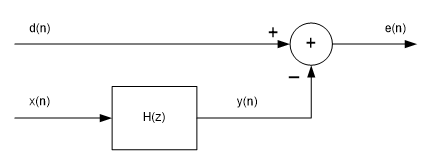
\includegraphics[width=0.5\textwidth]{images/wienerfiltering.png}
  \caption{维纳滤波噪声抑制系统框图}
  \label{fig:InterleavedFrequencies}
\end{figure}
\begin{itemize}
\item[$\bullet$] \textbf{输入信号}:含噪时段信号$x(n)$作为系统主输入
\item[$\bullet$] \textbf{期望信号}:$d_i(t)$通过排除第$i$时段的所有时段平均构建,以满足输入信号与期望信号不相关假设
\end{itemize}
\[ 
d_i(n) = \frac{1}{P} \sum_{\substack{j=0 \\ j \neq i}}^{P} x_j(n) 
\]
滤波器输出
\[ y_i(t) = \sum_{m=0}^{M-1} h_i(m)x_i(t-m) \]
其中 $h_i(m)$ 表示滤波器的冲激响应,其通过最小化误差信号的均方值求得:
这里误差信号 $e_i(n)$ 定义为:
\[
e_i(n) = d_i(n) - y_i(n)
\]
最优冲激响应是维纳-霍夫方程的解,其表达式为:
\[
\sum_{m=0}^{M-1} h_i(m) r_{x_i}(m-k) = p(-k), \quad k = 0,1,...,M-1
\]
其中:
\begin{itemize}
\item $r_{x_i}(m-k)$ 是输入信号的自相关函数
\item $p(-k)$ 是输入信号与期望信号的互相关函数
\end{itemize}

当噪声与目标信号的频谱重叠较小时,该方法效果最佳。
\subsection*{主成分分析与独立成分分析}
主成分分析(PCA)和独立成分分析(ICA)是两种信号处理方法,其目的是将波形分解为多个分量,并消除主要由噪声源产生的分量。
在PCA中,需要计算数据协方差矩阵的特征向量和特征值。对于n维数据集(n为ABR时间窗内的时间采样点数),共有n个特征向量。前几个分量包含信号的大部分方差,具有最大特征值的特征向量即为主成分。可根据特征值大小选择特征向量子集来重建信号。

ICA主要用于多通道分析,常用于处理EEG数据。若存在n个源信号,至少需要n个观测通道(即n个通道)才能获取原始信号。给定一组测量信号(即独立信号的混合),ICA通过变换产生具有最大非高斯性的独立分量信号。数据分解过程涉及从单通道头皮采集数据到空间变换"虚拟通道"基的线性转换。也就是说,数据从多个同步记录的单通道数据集合,转换为应用于整个多通道数据的空间滤波器的同步输出集合。
ICA将$n$维多元时间序列$\mathbf{x}$建模为$M$($M \leq n$)个统计独立源的线性组合。


给定$n$个线性混合信号和$n$个源信号:
\begin{itemize}
    \item 观测信号:$X_1, X_2, \ldots, X_n$
    \item 源信号:$S_1, S_2, \ldots, S_n$
\end{itemize}

\noindent 混合过程表示为:
\[
X_j = \sum_{k=1}^n a_{j,k}S_k \quad \text{其中}\; j = 1,2,\ldots,n
\]

\noindent 矩阵形式:
\begin{align*}
\mathbf{x} &= \mathbf{A}\mathbf{s} \quad \text{(混合方程)} \\
\mathbf{s} &= \mathbf{A}^{-1}\mathbf{x} = \mathbf{W}\mathbf{x} \quad \text{(分离方程)}
\end{align*}
\section{自动检测方法}
\subsection*{Hotelling's T²}
Hotelling's T²统计量用于多元假设检验。在“不存在响应信号”的零假设条件下,该方法通过计算数据样本任意线性组合的均值与零的显著性差异概率来进行统计推断。

在ABR检测中的具体应用步骤如下:首先对信号进行1500Hz低通滤波预处理;随后将感兴趣信号区域划分为10个时间仓(每个仓宽0.45ms)——对于75dB感觉级刺激的响应从5.5ms开始分段,40 dB 感觉级刺激则从8.5ms开始;接着计算各时间仓内的信号平均值;最终每个时段提取10个特征点作为T²分析的输入数据。
\[
T^2 = N(\bar{\mathbf{x}} - \boldsymbol{\mu})^\top \mathbf{S}^{-1}(\bar{\mathbf{x}} - \boldsymbol{\mu})
\]

其中:
\begin{itemize}
    \item $N$:扫描次数
    \item $\bar{\mathbf{x}}$:平均数据向量
    \item $\boldsymbol{\mu}$:零假设下的总体均值向量(本文中$\boldsymbol{\mu} = \mathbf{0}$)
    \item $\mathbf{S}$:$p \times p$维数据协方差矩阵
\end{itemize}

T$^2$统计量可通过以下关系转换为F分布:
\[
\frac{(N - p)T^2}{(N - 1)p} \approx F_{(p, N - p)}
\]
因此,可以确定存在响应信号的概率。
\subsection*{F$_{sp}$方差比}
F$_{sp}$方差比是检测 ABR 信号的标准方法,尤其适用于新生儿听力筛查。该指标通过计算以下方差比实现:

\[
\text{F}_{sp} = \frac{\sigma^2_{\text{信号}}}{\sigma^2_{\text{噪声}}}
= \frac{\mathrm{var}(\overline{X})}{\mathrm{var}(SP)}
\]
\[
\mathrm{var}(\overline{SP}) = \frac{\mathrm{var}(SP)}{N}
\]

\begin{itemize}
    \item \textbf{分子}:多次扫描平均波形的幅值方差
    \item \textbf{分母}:固定时间点处各扫描幅值的方差
\end{itemize}
翻译如下:

用于计算 F$_{sp}$ 的时间窗口的大小和位置可以根据刺激类型、呈现强度以及感兴趣波形特征的潜伏期进行调整。基于获得的 ABR 记录数据,以及主要关注的是检测 V–V' 波的存在与否,因此 F$_{sp}$的计算可以使用一个以 V 波为中心的较短时间窗口。在本研究中,使用的时间窗口为刺激后 7–11 毫秒(对应 75 dB SL)或 8–12 毫秒(对应 40 dB SL)。

 F$_{sp}$  与信噪比之间的关系如下:
\[
F_{SP} = \left[ SNR^2 + 1 + 2 \cdot R(EP, \overline{BN}) \cdot SNR \right] \cdot \frac{\mathrm{var}(\overline{BN})}{\mathrm{var}(\overline{SP})}
\]
方差比遵循 $F$ 分布 \( F(v_1, v_2) \),其中 \( v_1 \) 和 \( v_2 \) 分别是分子和分母的自由度。如果背景噪声是真正的白噪声,那么自由度 \( v_1 \) 应等于时间窗内的采样点数。然而,噪声的带宽越窄,自由度 \( v_1 \) 越低,因此该值需要进行估计。本文使用了一个非常保守的估计,即 \( v_1 = 5 \)。

分母的自由度 \( v_2 \) 是试次数 \( N \)。

根据 $F$ 分布查找表 \( F_{(5, 250)} \),95\% 置信水平的阈值为 2.25,99\% 置信水平的阈值为 3.1。在新生儿听力筛查中,通常使用F$_{sp}$ 值为 3.1 作为通过/未通过的判定标准。

由于在样本量较小的情况下,单点方差并不能准确估计背景噪声的方差,因此在本研究中, F$_{sp}$  比值的分母是基于时间窗内全部 \( J \) 个采样点所计算的方差,并对结果进行了平均处理。
\[
F_{SP} = \frac{\text{var}(S)}{\frac{1}{J}\sum_{j=1}^{J}\text{var}(\overline{SP}_{j})}
\]
\subsection*{方差比点(POVR)}
POVR与  F$_{sp}$ 类似,但其分子部分的方差更大,因为仅使用响应中的部分时间点(如4或10个点),而非全部数据点(Sininger等,2001)。所选时间点通过最大化目标/模板波形的方差来确定,通常包括目标波形的最大峰值和最小峰值(对于ABR,可能是波III、波V或波V')。

由于波形形态会因刺激类型、速率、呈现强度、电极位置和受试者年龄等因素而变化,可以预见,不同刺激条件下可能需要不同的模板或时间点。此外,若个体存在峰值潜伏期偏移,检测功效也会降低。

\section{实验与结果}
\subsection*{刺激集}
呈现的完整刺激集包括:
\begin{table}[H]
\centering
\caption{听觉刺激参数表}
\label{tab:stimulus_params}
\begin{tabular}{llll}
\toprule
\textbf{刺激类型} & \textbf{极性/频率} & \textbf{呈现速率} & \textbf{强度(dB SL)} \\
\midrule
\hline
Click & 稀疏(Rarefaction) & 10, 20 Hz & 75, 40 \\
     & 凝聚(Condensation) &          &   \\
\hline
单调音(Tone) & 4000 Hz  &       & 75, 40 \\
            & 500 Hz              &       & \\
            & 500 Hz(交替极性)    &       & 75, 40 \\
\hline
M-Chirp & 100–10400 Hz & 20 Hz & 75, 40 \\
\hline
Octave Chirp & 4000 Hz &       &           \\
                      & 500 Hz  &       &           \\
\hline
\multirow{5}{*}{MLS} & Click        & 250 Hz, 300 Hz & 75, 40 \\
                                   & 500 Hz Tone   & 250 Hz         & 75, 40 \\
                                   & 4000 Hz Tone  &   &  \\
                                   & 500 Hz Chirp   &    &  \\
                                   & 4000 Hz Chirp  &    &  \\
\hline
交错频率 & Tone4k,2k,1k,500Hz& Tone18ms,序列55ms & 75, 40 \\
        & Chirp4k,2k,1k,500Hz& &    \\
\hline
GHINOMA & Tone4k,2k,1k,500Hz&       & 65 \\
        & Chirp4000,2000,1000,500Hz &       &   \\
\bottomrule
\end{tabular}
\end{table}

\subsection*{实验设置}
Neuroscan EEG系统是专业脑电采集平台,广泛应用于临床神经生理学和认知神经科学研究。系统以高精度信号采集和灵活的配置著称,支持从常规脑电到事件相关电位(ERP)的全方位研究需求。

\begin{figure}[H]
\centering
% 左表格:系统参数
\begin{minipage}[t]{0.48\textwidth}
\centering
\captionof{table}{系统硬件参数} % 添加的标题
\adjustbox{valign=t}{
\begin{tabular}{>{\bfseries}ll}
\toprule
\textbf{参数} & \textbf{设置值} \\
\midrule
A/D采样率 & 20,000 Hz \\
增益 & 2500 \\
高通滤波 & 100 Hz \\
低通滤波 & 3000 Hz \\
采样模式 & Continuous \\
伪迹剔除阈值 & ±50 μV \\ % 补充单位说明
\bottomrule
\end{tabular}
}
\label{tab:hardware_params}
\end{minipage}
\hfill
% 右表格:电极配置
\begin{minipage}[t]{0.48\textwidth}
\centering
\captionof{table}{电极配置方案} % 添加的标题
\adjustbox{valign=t}{
\begin{tabular}{>{\bfseries}l>{\ttfamily}l}
\toprule
\textbf{通道} & \textbf{导联设置(电极位置)} \\ % 修改列名
\midrule
通道1 & Cz → Inion (顶点→枕骨隆突) \\
通道2 & Cz → A1 (顶点→左耳垂) \\
通道3 & T1 → T2 (左颞→右颞) \\ % 统一缩写
通道4 & T1 → A1 (左颞→左耳垂) \\ % 补充说明
\addlinespace
刺激呈现 & 插入式耳机 \\
\bottomrule
\end{tabular}
}
\label{tab:electrode_config}
\end{minipage}
\end{figure}

\subsection*{刺激综合对比与实验}
\subsubsection{ABR信号与噪声频谱}
展示了不同受试者在无刺激状态下的频率频谱特征。通过短时傅里叶变换(STFT)对3分钟连续记录信号进行分析,采用102.4毫秒50\%重叠汉明窗,最终对幅值频谱进行平均处理。50Hz频谐波成分显著存在,尤以Cz-Inion导联通道最为明显。

\begin{figure}[H]
  \centering
  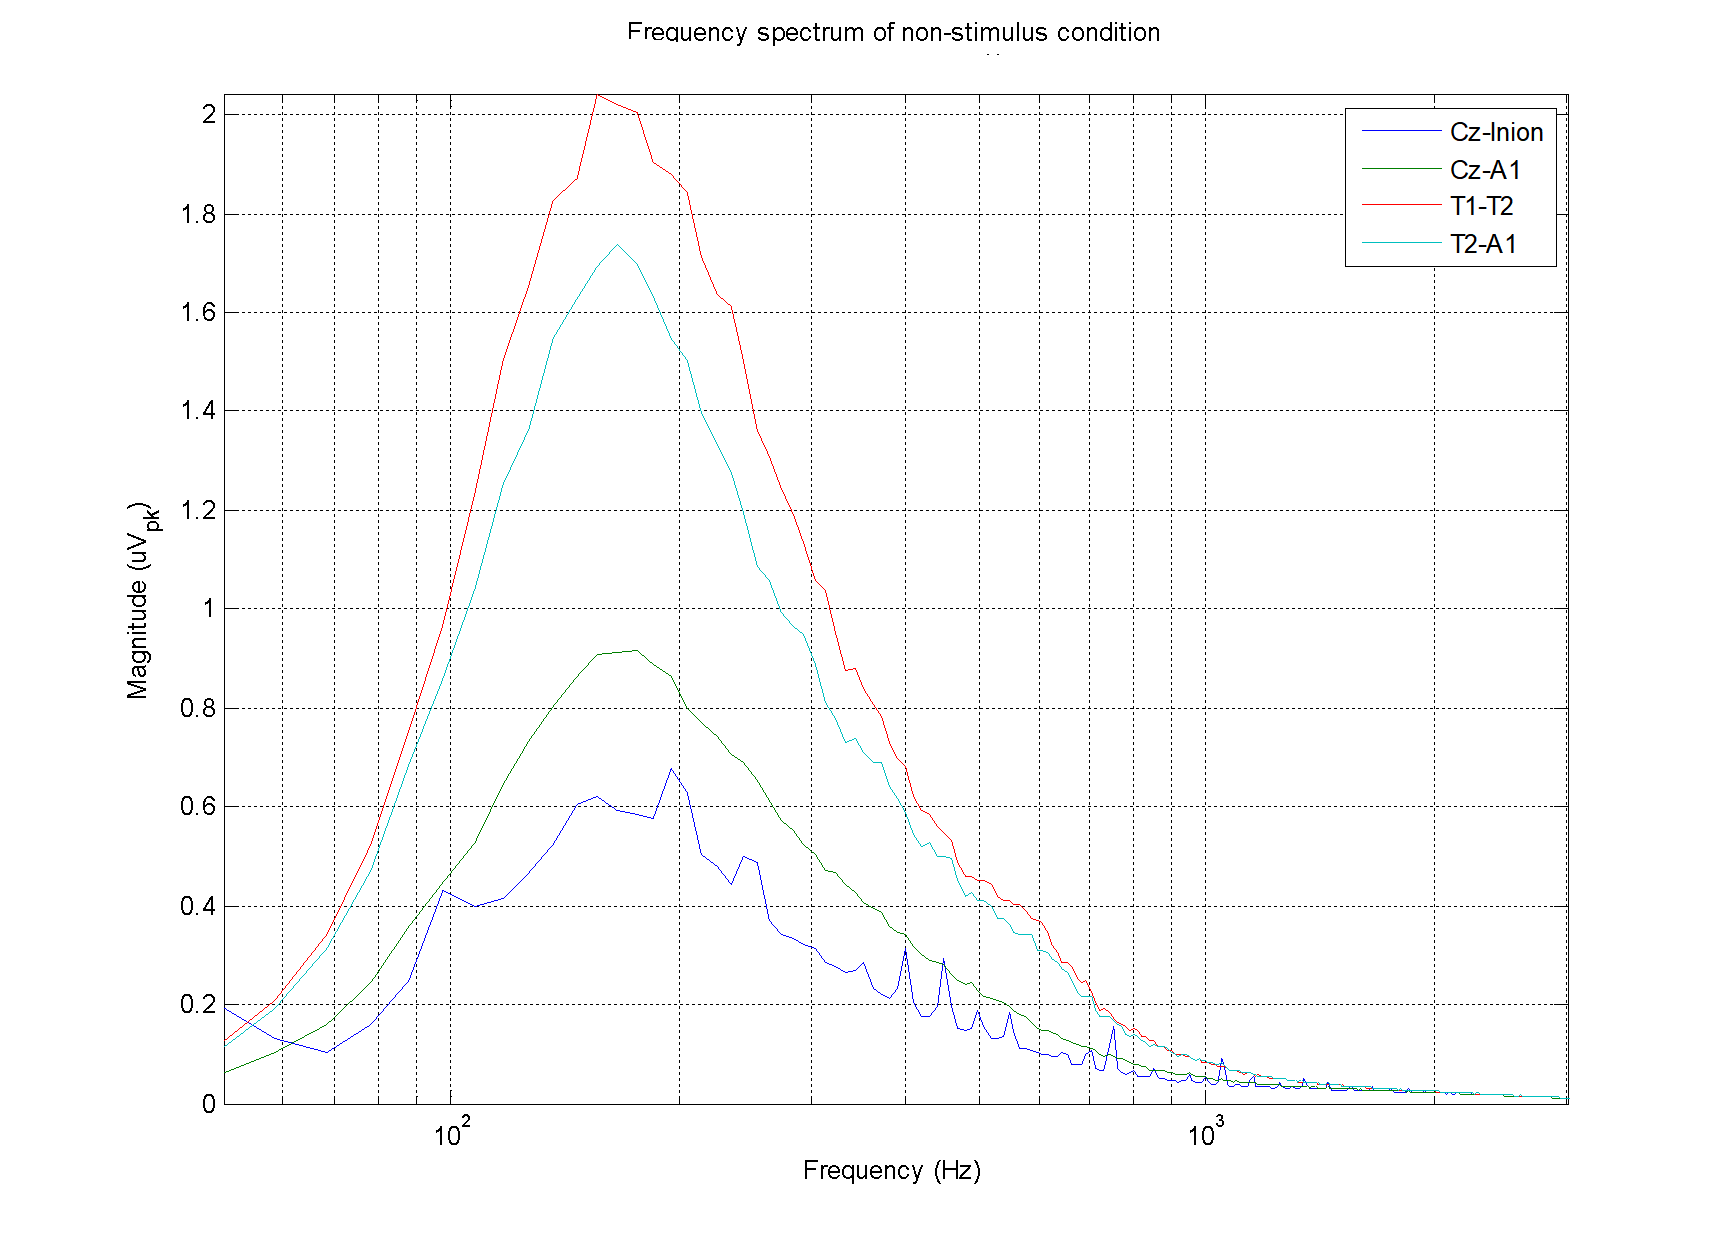
\includegraphics[width=0.5\textwidth]{images/FrequencyspectrumOfNon-StimulusCondition-1.png}
  \caption{噪声频谱}
  \label{fig:FrequencyspectrumOfNon-Stimulus}
\end{figure}
\subsubsection{通过波形平均改善信噪比}
作为基础处理步骤,所有ABR记录均经过以下预处理:
带通滤波(100-3000 Hz), 分段对齐(分析时窗15-25 ms),信号平均处理

下两图展示了定期计算的平均波形结果。随着叠加次数(Sweeps)的增加,ABR特征波的峰潜伏期界定愈加清晰。
\begin{figure}[H]
    \centering
    \begin{minipage}{0.48\textwidth}
        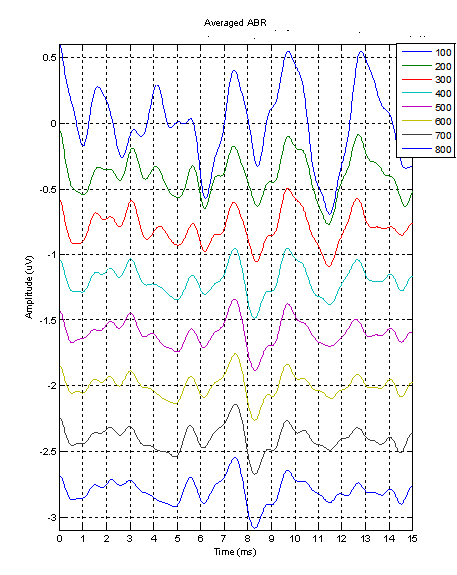
\includegraphics[width=\textwidth]{images/improvingSNRwaveformAveraging75.png}
    \end{minipage}
    \hfill
    \begin{minipage}{0.48\textwidth}
        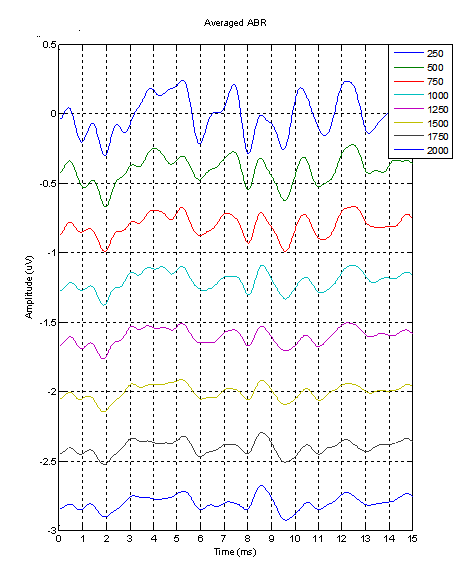
\includegraphics[width=\textwidth]{images/improvingSNRwaveformAveraging40.png}
    \end{minipage}
\end{figure}
在75 dB刺激强度下,受试者的短声刺激诱发波V潜伏期为7.2±0.3 ms,较已发表的标准值6.4±0.2 ms(使用插入式耳机时为5.6 ms+0.8 ms)偏高,可能与Neuroscan系统的触发同步时序问题有关。当改用500 HzTone刺激时,波V潜伏期延长至9.0±0.4 ms(相同强度)。

当刺激强度降至40 dB SL时,短声刺激的波V潜伏期为8.41±0.3 ms,而500 HzTone刺激则进一步延长至约10.8 ms。值得注意的是,低频Tone刺激在仅叠加2000次时,波V成分常难以通过视觉检测确认。

信号处理方法比较
通过 F$_{sp}$值评估了常规平均、加权平均和分块加权平均三种方法的性能如下图。由于受试者保持高度安静状态且记录期间背景噪声稳定,加权处理未显现优势。有趣的是,虽然Cz-Inion导联记录的波V-V'振幅较大,但其背景噪声水平显著高于Cz-A1导联,导致 F$_{sp}$比值明显降低。


\begin{figure}[H]
    \centering
    \begin{minipage}{0.48\textwidth}
        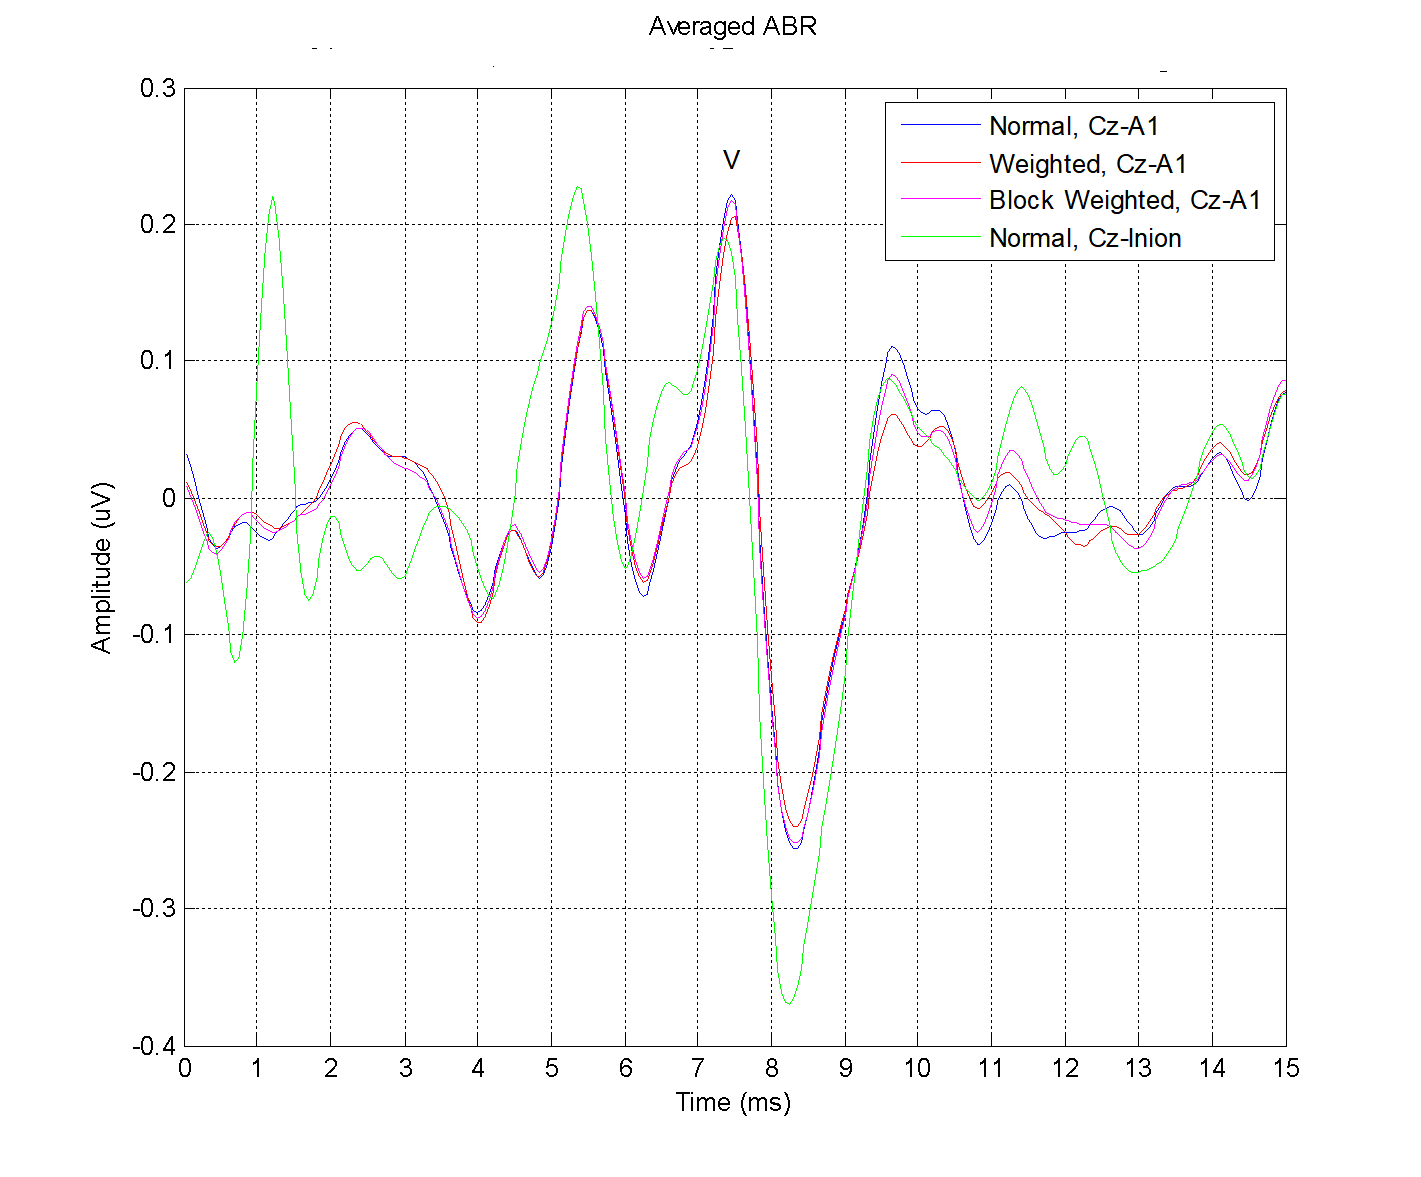
\includegraphics[width=\textwidth]{images/click75dbABR.png}
    \end{minipage}
    \hfill
    \begin{minipage}{0.48\textwidth}
        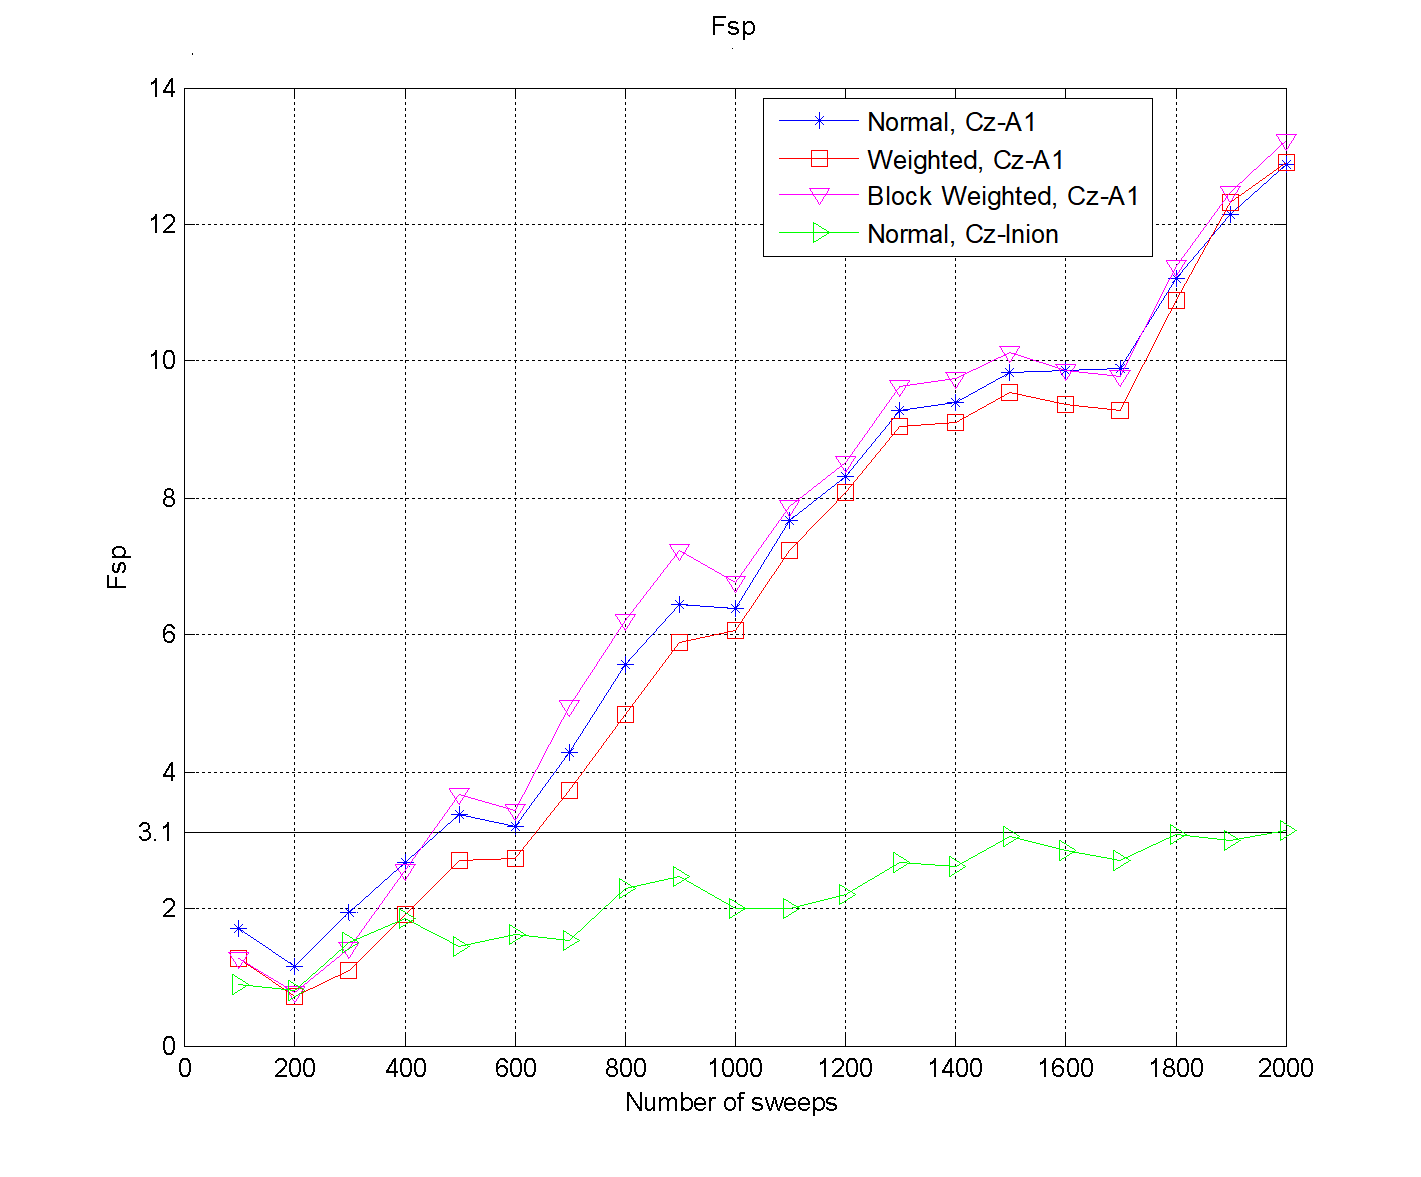
\includegraphics[width=\textwidth]{images/click75dbABRfsp.png}
    \end{minipage}
    
    \vspace{0.2cm}
    
    \begin{minipage}{0.48\textwidth}
        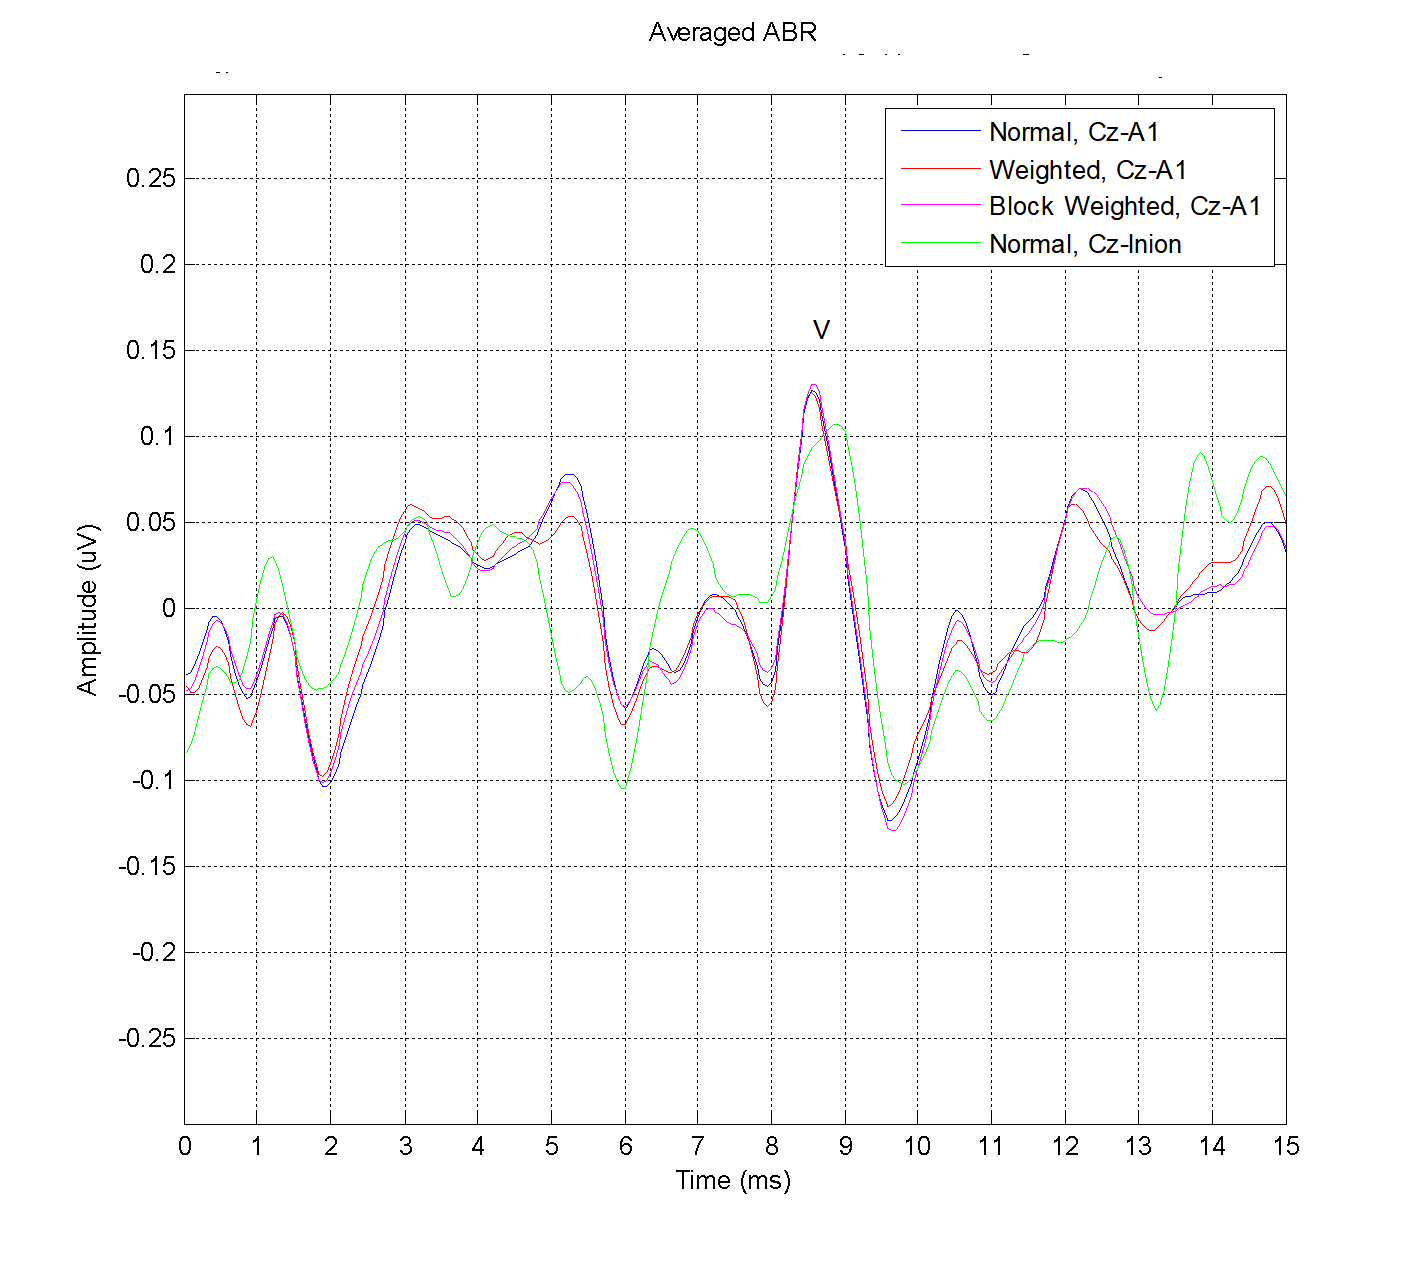
\includegraphics[width=\textwidth]{images/click40dbABR.png}
    \end{minipage}
    \hfill
    \begin{minipage}{0.48\textwidth}
        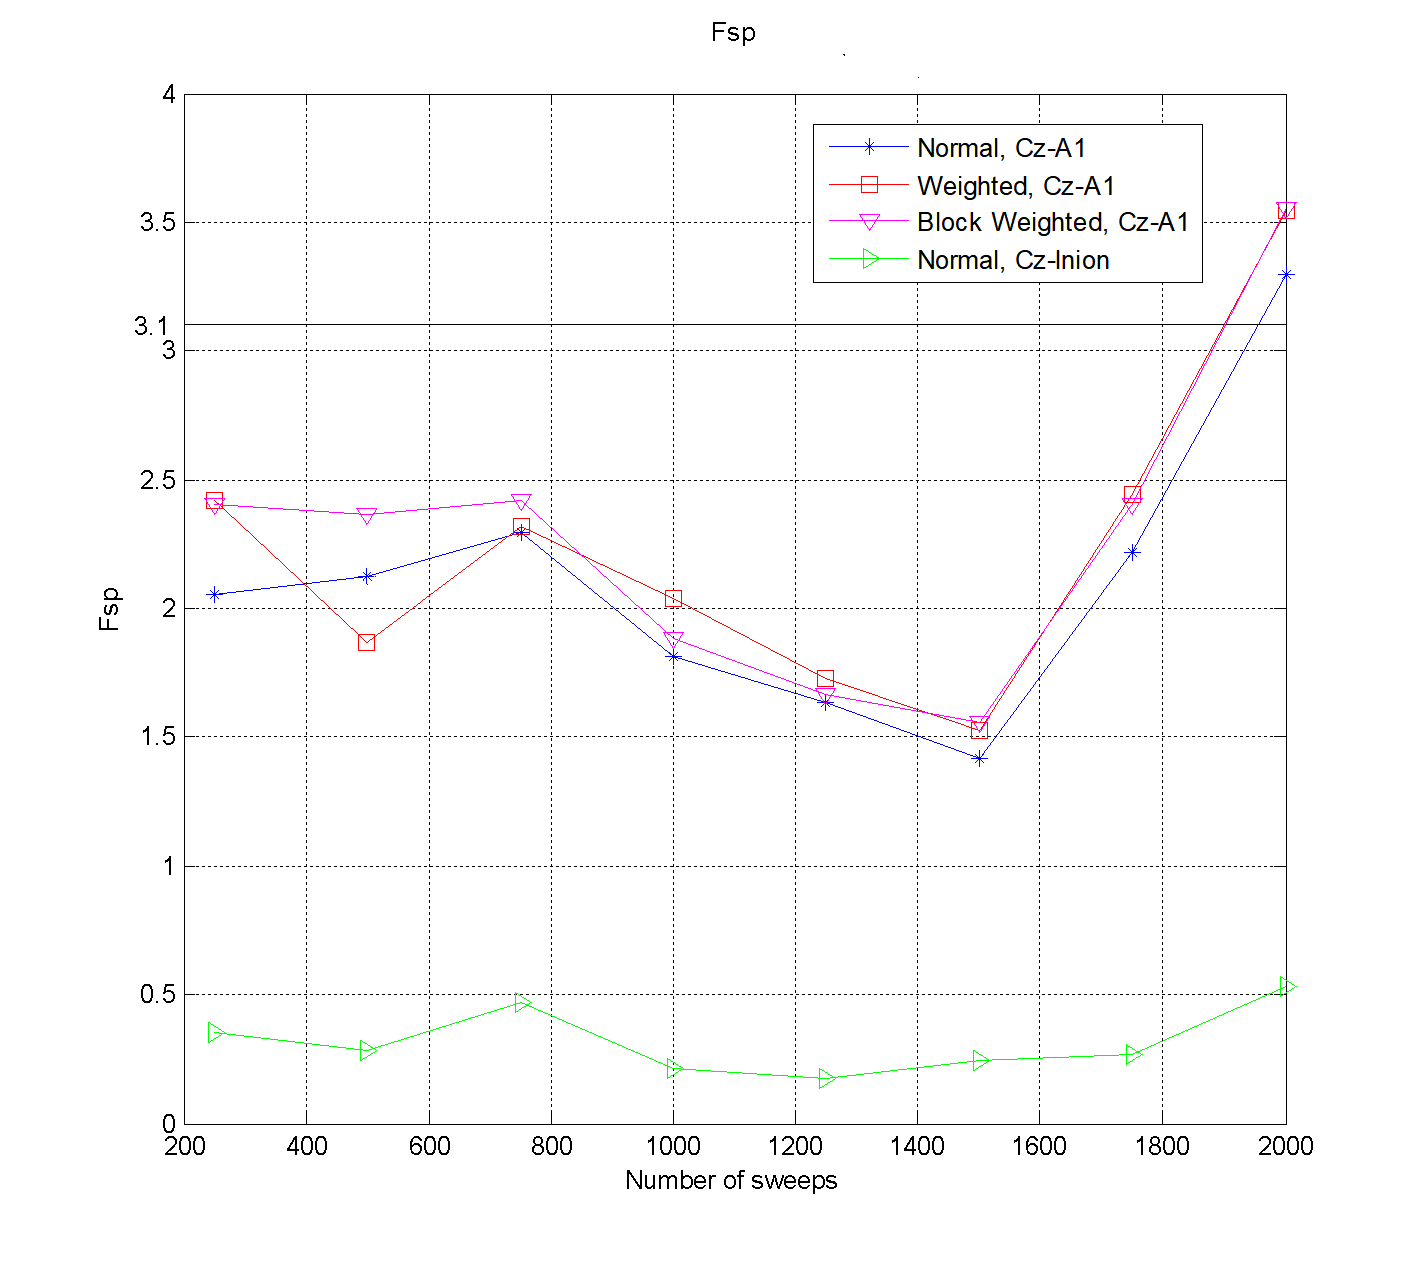
\includegraphics[width=\textwidth]{images/click40dbABRfsp.png}
    \end{minipage}
    \caption{常规平均、加权平均和分块加权平均在75,40 dB的潜伏期和性能}
    \label{fig:7540ABRAndFsp}
\end{figure}

\subsubsection{Chirp刺激诱发的响应}
\paragraph{宽带Chirp}
在40 dB SL刺激强度下,受试者的波V-V'峰峰值振幅显著增强,而在75 dB SL下振幅反而降低。

Chirp刺激在低刺激强度(20–40 dB SL)下的增强效应与Dau等(2000)\cite{dau2000optimized}的研究一致,该研究发现波V振幅在低强度下显著增大,但在50–60 dB SL时无此优势。这可能是因为高强度刺激下,低频能量同时刺激耳蜗基底区,导致神经反应同步性降低,部分抵消了重叠响应峰的增强效果。
\begin{table}[H]
\centering
\caption{不同刺激条件下波V-V'振幅及Chirp刺激改善率}
\label{tab:wave_amplitude}
\begin{tabular}{llcc}
\toprule
\multicolumn{1}{c}{\textbf{刺激强度}} & \multicolumn{1}{c}{\textbf{刺激类型}} & \textbf{波V-V'振幅 (uV)} & \textbf{改善率} \\
\midrule
\multirow{6}{*}{75 dB SL} & \multicolumn{3}{l}{\textbf{受试者 LC}} \\
 & Click (负极性) & 0.36 & \\
 & Click (正极性) & 0.45 & \\
 & Chirp & 0.27 & -(27-41)\% \\
\cmidrule{2-4}
 & \multicolumn{3}{l}{\textbf{受试者 DR}} \\
 & Click (负极性) & 0.46 & \\
 & Click (正极性) & 0.47 & \\
 & Chirp & 0.25 & -46 \\
\midrule
\multirow{6}{*}{40 dB SL} & \multicolumn{3}{l}{\textbf{受试者 LC}} \\
 & Click (负极性) & 0.22 & \\
 & Click (正极性) & 0.17 & \\
 & Chirp & 0.46 & +(100-156)\% \\
\cmidrule{2-4}
 & \multicolumn{3}{l}{\textbf{受试者 DR}} \\
 & Click (负极性) & 0.23 & \\
 & Click (正极性) & 0.13 & \\
 & Chirp & 0.32 & +(33-146)\% \\
\bottomrule
\end{tabular}
\smallskip
\footnotesize
\textsuperscript{*} 改善率计算基于与同条件下最优Click刺激值的比较,范围值表示不同极性刺激的对比结果
\end{table}
\newpage
\paragraph{特定频率Chirp}
针对4000 Hz和500 Hz频率的刺激,比较了窄带Chirp刺激引起的反应与Tone刺激引起的反应。
\begin{figure}[H]
    \centering
    \begin{minipage}{0.48\textwidth}
        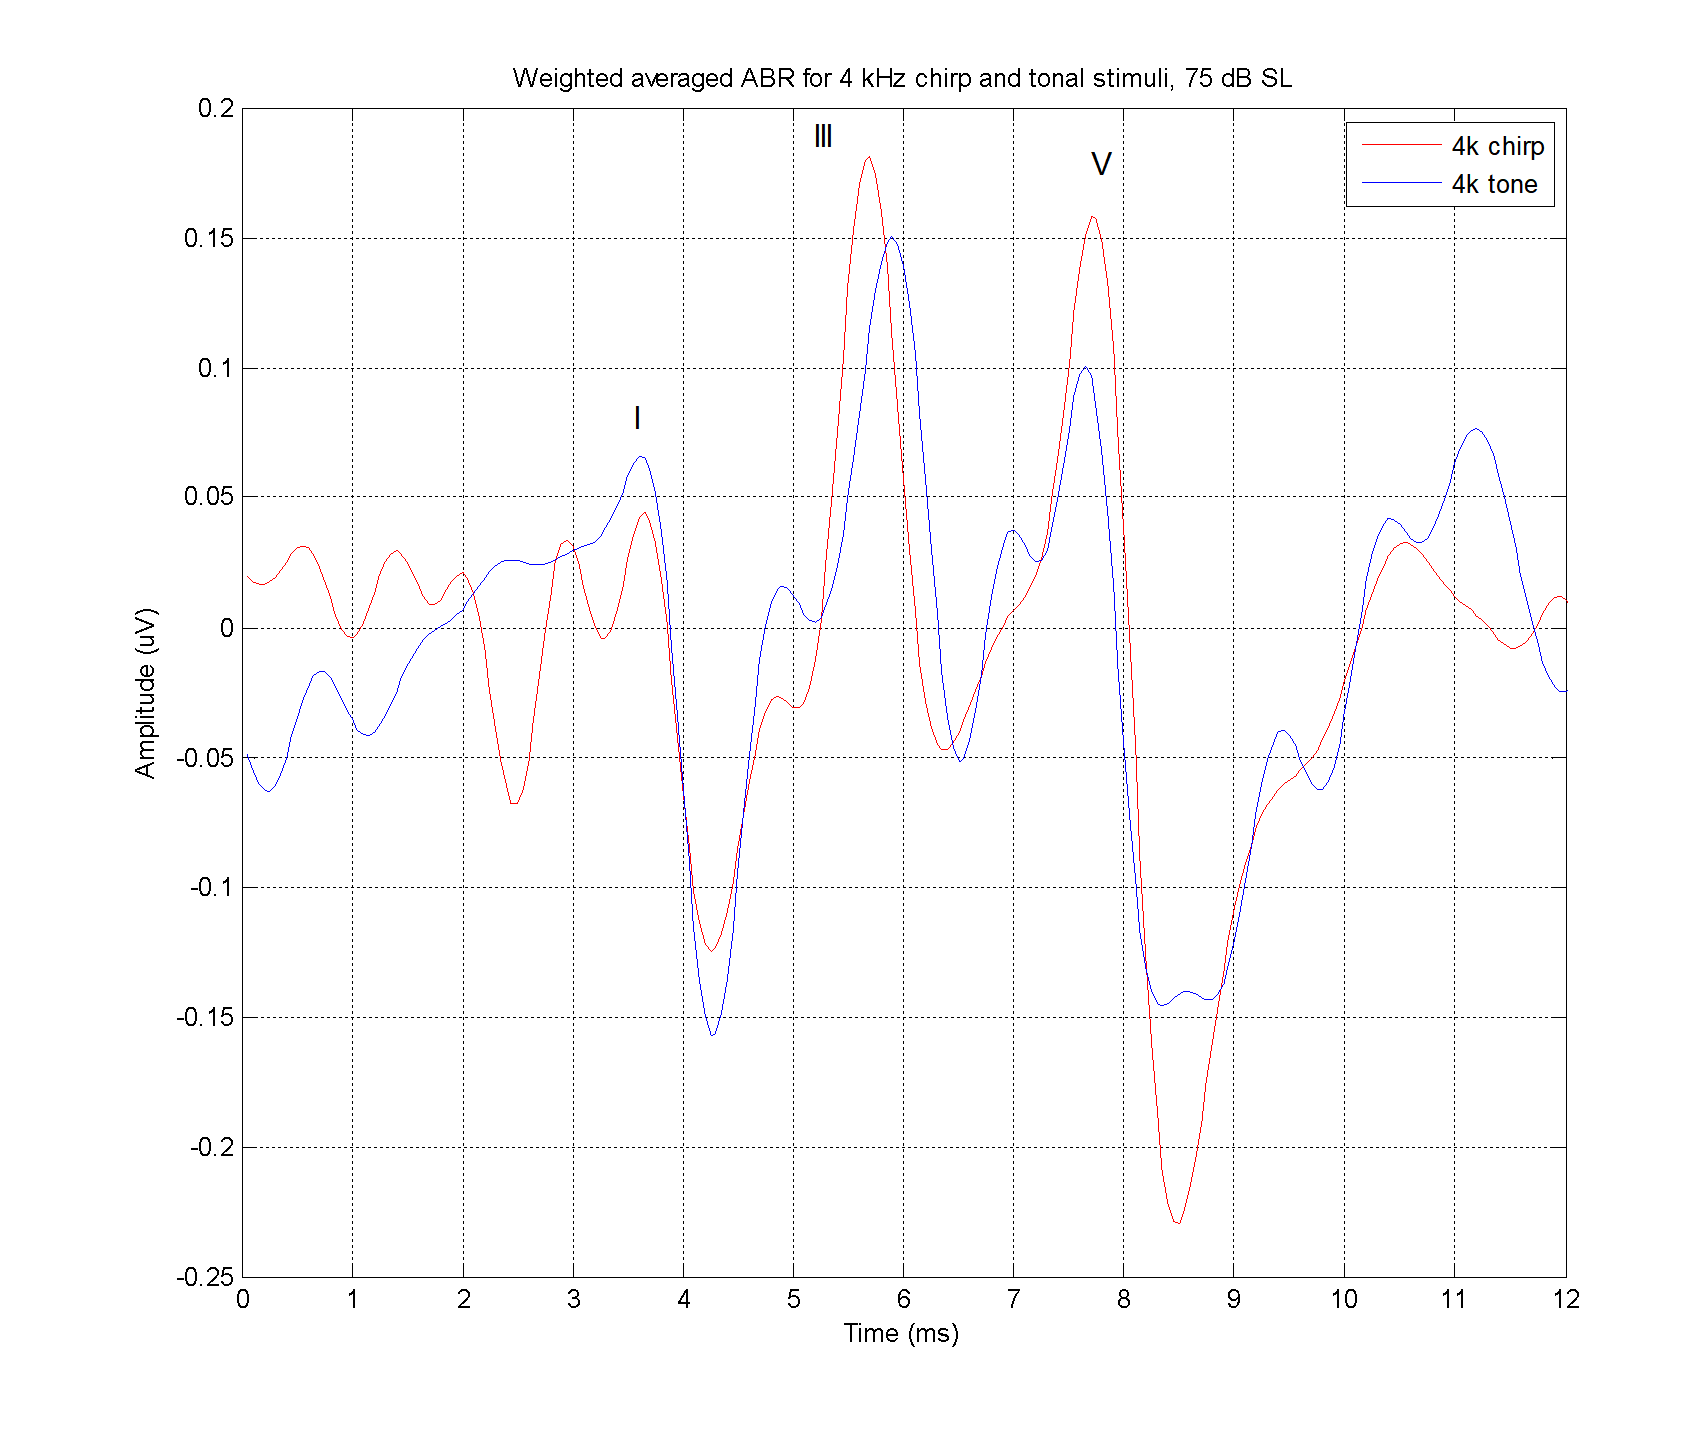
\includegraphics[width=\textwidth]{images/4kchirpAndTonalStimuli75db.png}
    \end{minipage}
    \hfill
    \begin{minipage}{0.48\textwidth}
        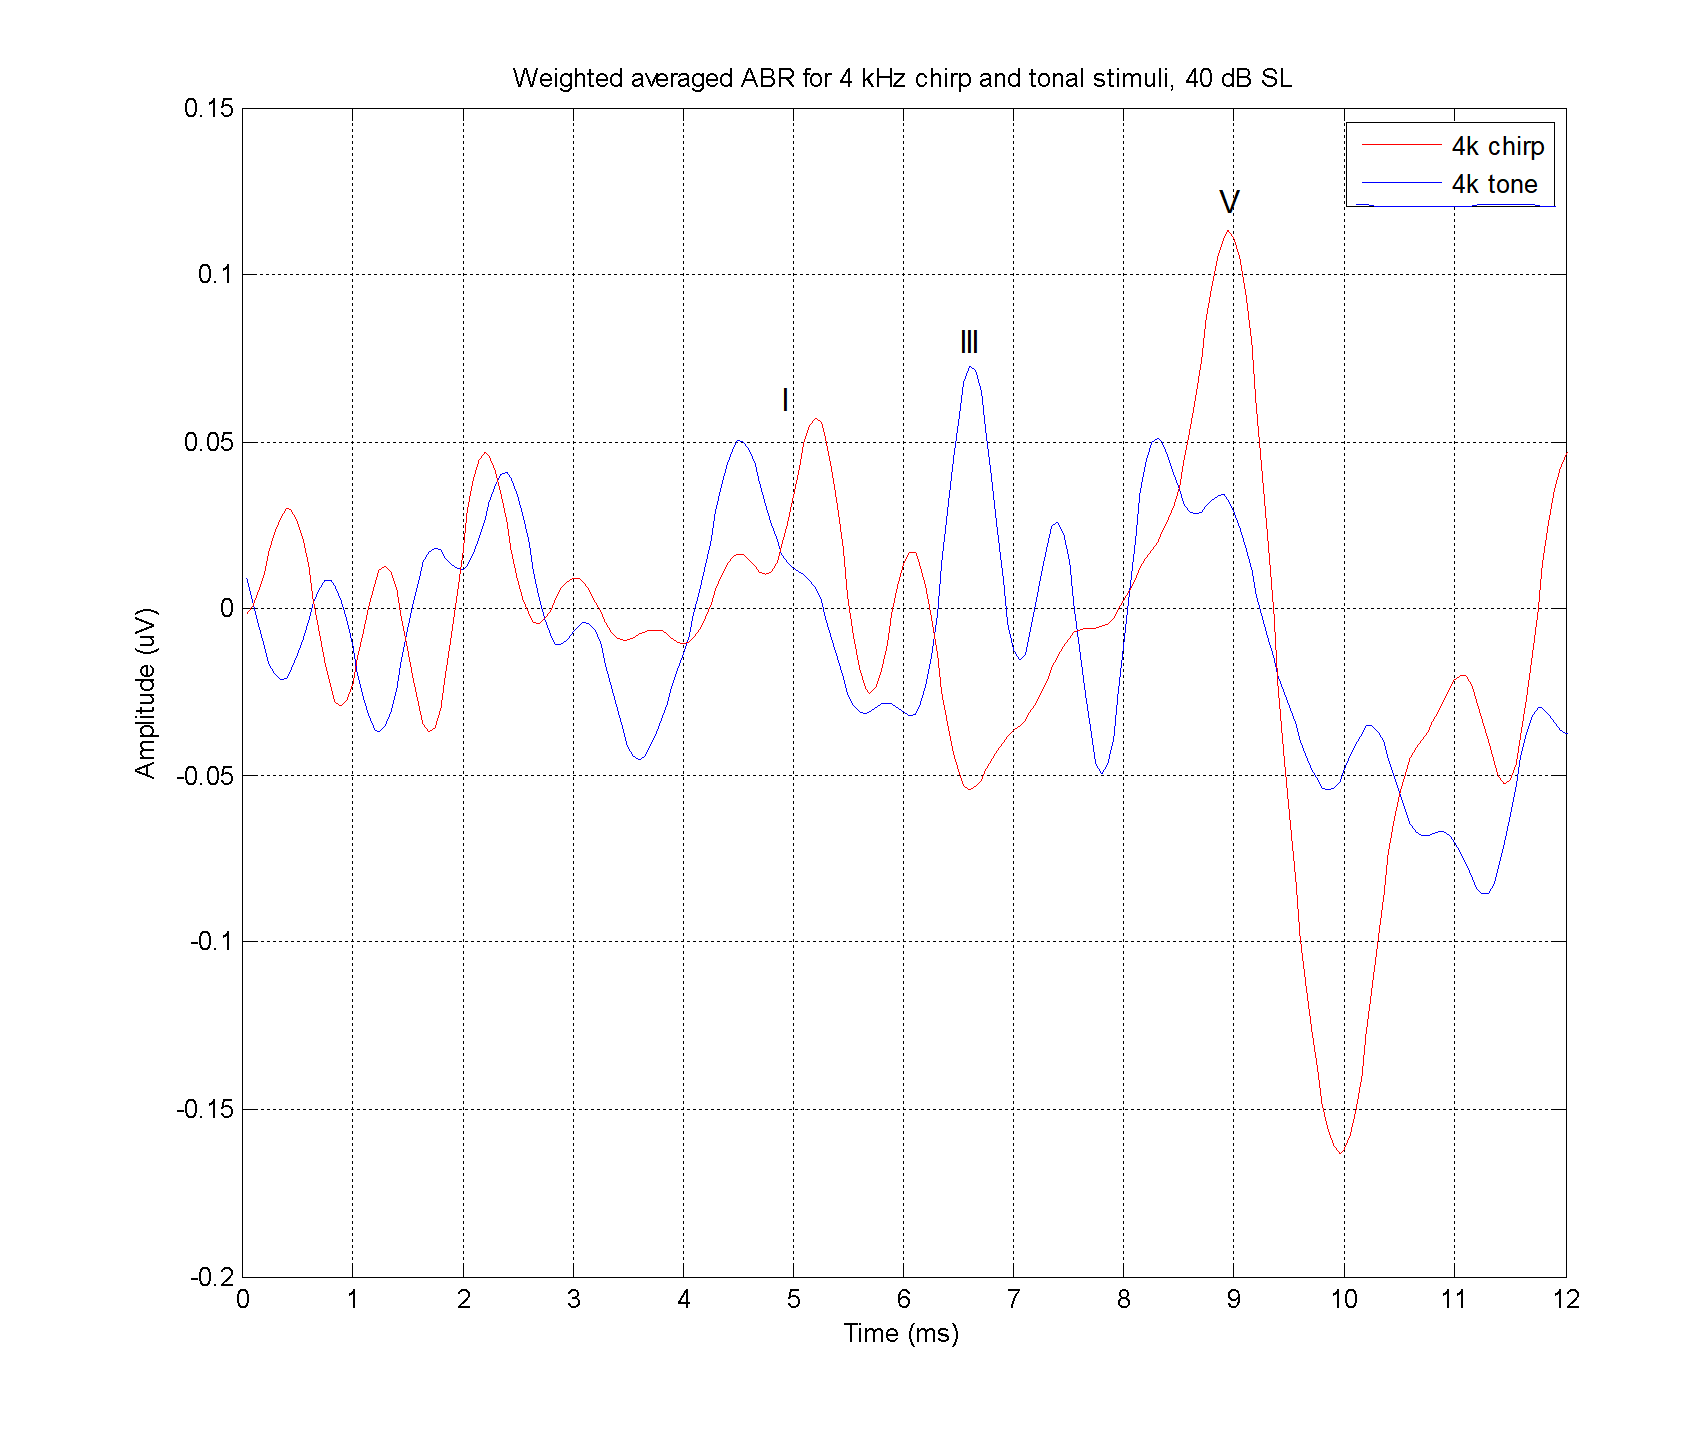
\includegraphics[width=\textwidth]{images/4kchirpAndTonalStimuli40db.png}
    \end{minipage}
    
    \vspace{0.2cm}
    
    \begin{minipage}{0.48\textwidth}
        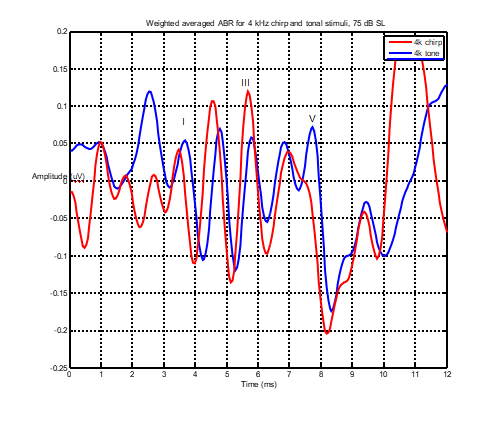
\includegraphics[width=\textwidth]{images/4kchirpAndTonalStimuli75db2.png}
    \end{minipage}
    \hfill
    \begin{minipage}{0.48\textwidth}
        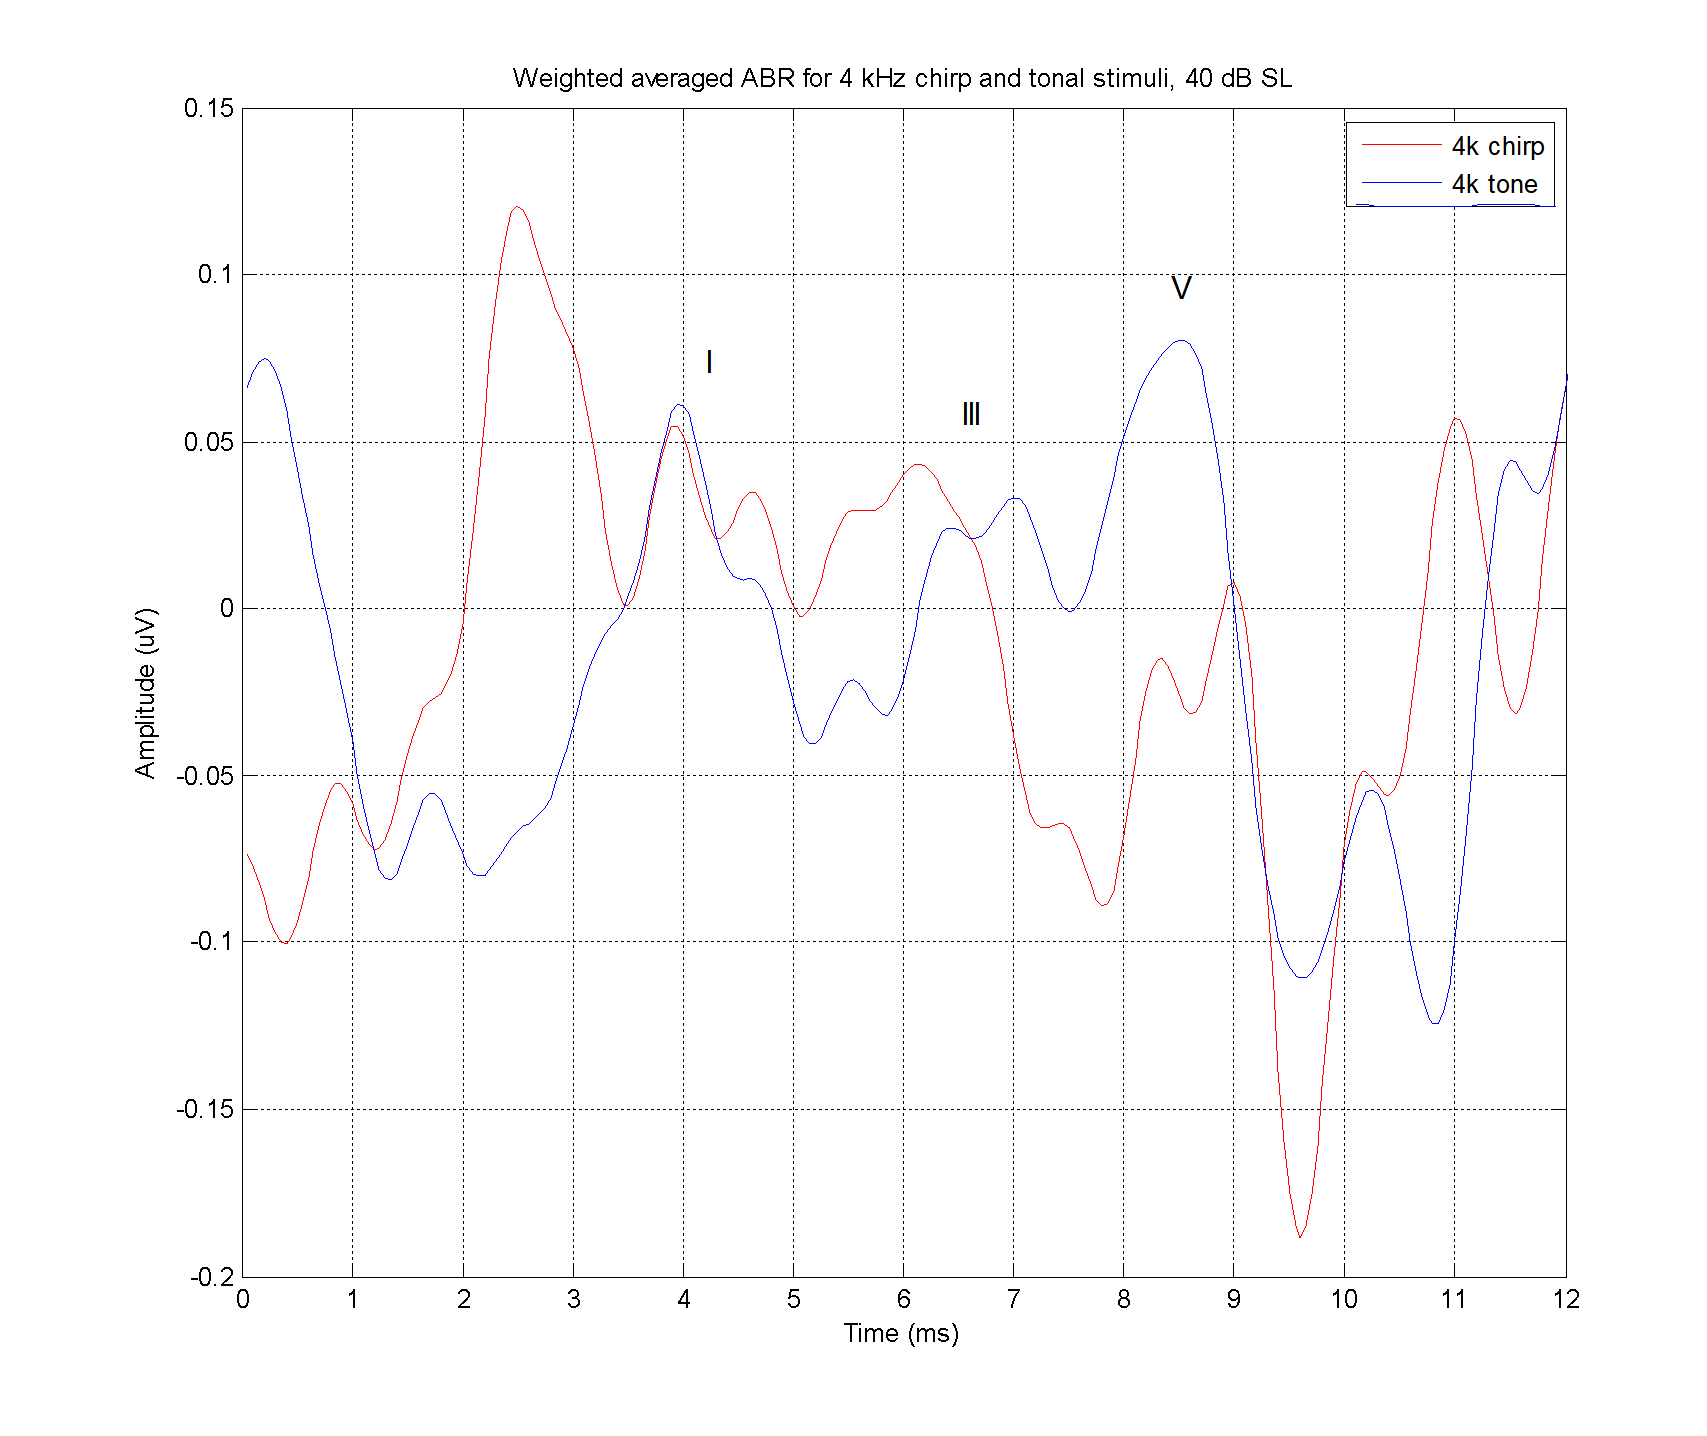
\includegraphics[width=\textwidth]{images/4kchirpAndTonalStimuli40db2.png}
    \end{minipage}
    \caption{两个测试者的4 kHz 窄带Chirp声和Tone刺激}
    \label{fig:twotester4kchirpandtone}
\end{figure}
对于受试者1,在75 dB SL强度下,Chirp声刺激诱发的V波振幅为156 nV,Tone刺激为100 nV,增幅达56\%。在40 dB SL强度下,效果更为显著:Chirp声刺激的V波振幅为110 nV,Tone刺激仅50 nV(增幅120\%)。
对于受试者2,无论是75 dB SL还是40 dB SL强度,Chirp声与Tone刺激的V波峰峰值(V-V’)振幅均基本一致。

与4 kHz刺激响应相比500 HzTone刺激经过2000次叠加后的平均响应表现出显著更高的噪声水平。无论是75 dB SL还是40 dB SL强度,Chirp刺激诱发的波V振幅与Tone刺激相比均呈现相似或降低的趋势。值得注意的是,受试者1在40 dB SL强度下的响应未出现预期的峰值/潜伏期特征(可能源于记录误差或过量噪声),该数据已在后续分析中剔除。

\textbf{主要发现:}
Chirp刺激对波V振幅的提升效果在不同受试者及刺激频率间缺乏一致性。然而总体而言,研究证实Chirp刺激在以下方面具有优势:

宽带频率响应检测

4 kHz高频信号采集

低刺激强度(≤40 dB SL)条件下的信号增强

\subsubsection{交错频率刺激的响应特征}
本研究采用含噪声掩蔽(GHINOMA)和无掩蔽条件的交错频率Tone/Chirp刺激序列(4000、2000、1000、500 Hz)采集数据。
\paragraph*{无噪声掩蔽刺激序列参数}

实验采用精确定时的多频刺激序列设计:\textbf{时序参数}设置包含高频至低频的切换间隔(18 ms)和序列循环间隔(50 ms,位于500 Hz刺激后),据此计算得总周期时长$T_{\text{total}} = 3 \times 18,\text{ms} + 50,\text{ms} = 104,\text{ms}$。\textbf{刺激效率}通过有效速率公式$R_{\text{eff}} = \frac{1000}{104,\text{ms}/4} \approx 38.5,\text{Hz}$确定,在5秒记录时长内可完成$5,\text{s} \times 38.5,\text{Hz} = 192$次扫描。该设计通过$\frac{104,\text{ms}}{\text{周期}}$的紧凑时序实现了频段间的快速切换与信号的高效采集。
\begin{figure}[H]
    \centering
    \begin{minipage}{0.48\textwidth}
        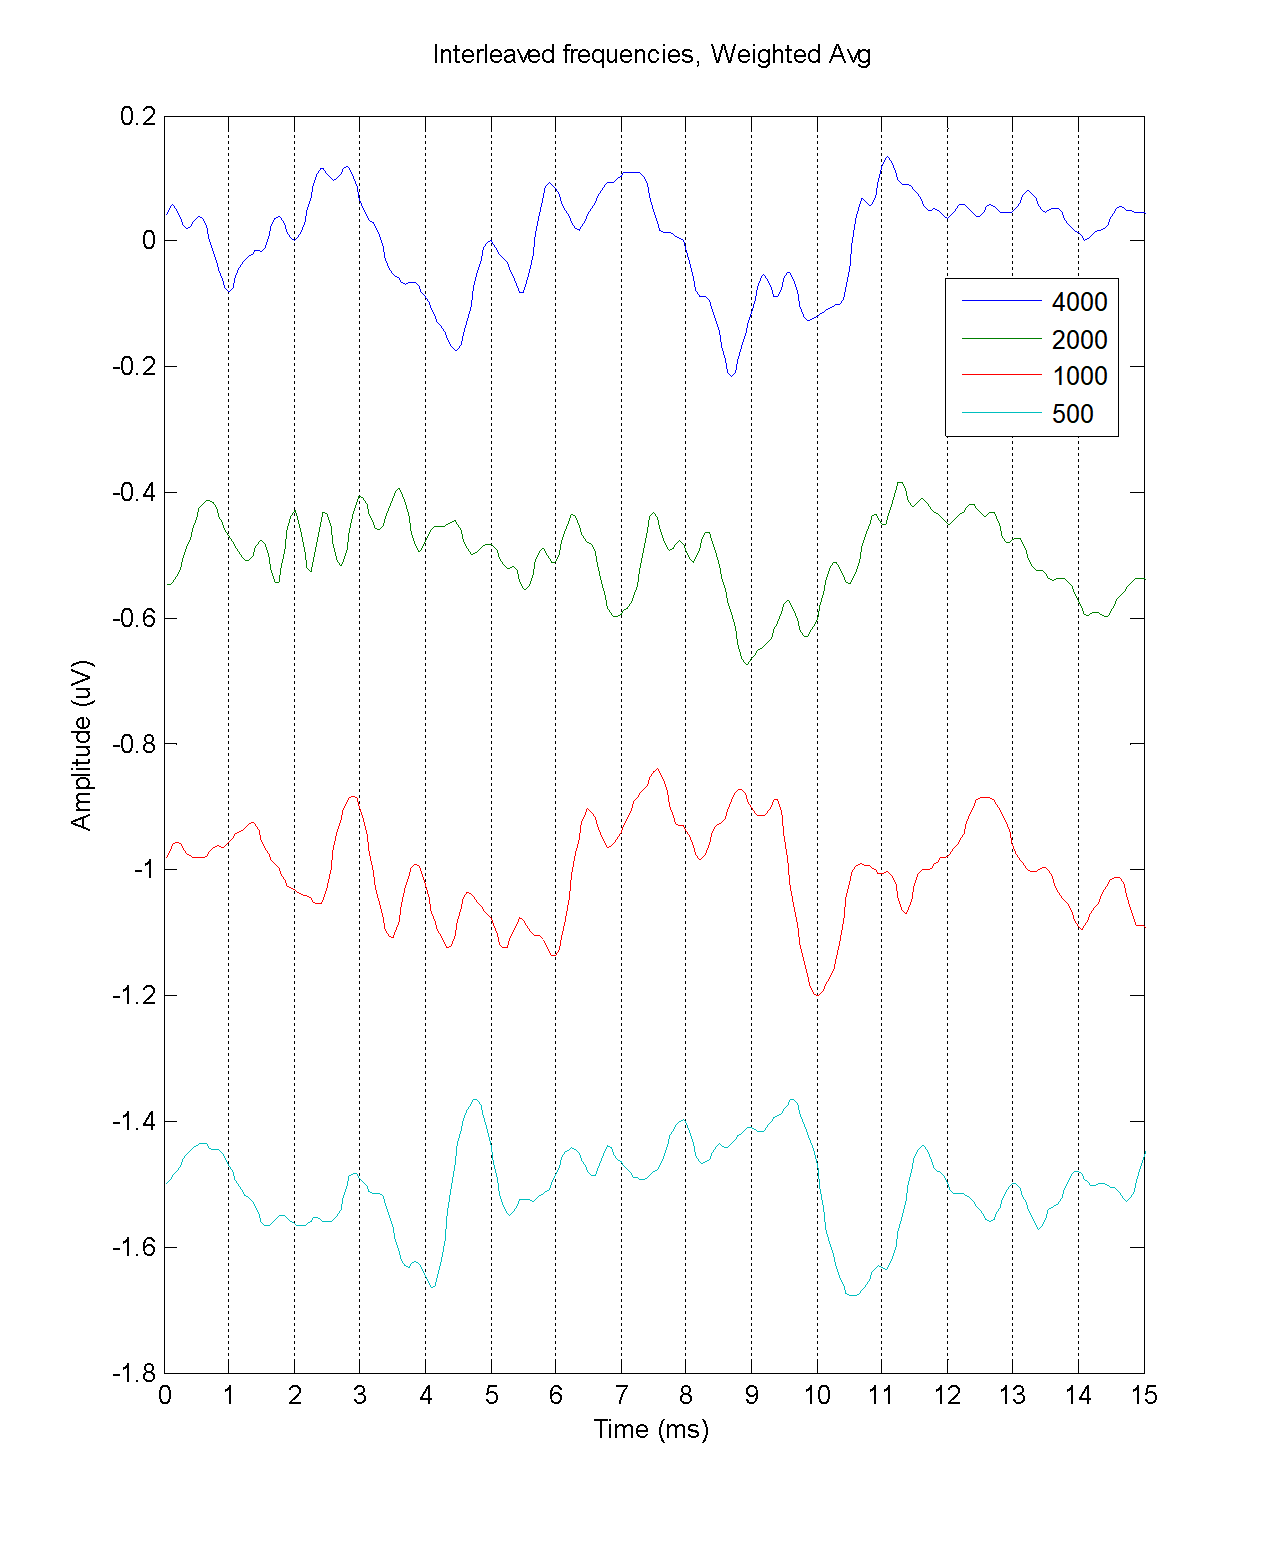
\includegraphics[width=\textwidth]{images/Interleaved75dbGHINOMA-1.png}
    \end{minipage}
    \hfill
    \begin{minipage}{0.48\textwidth}
        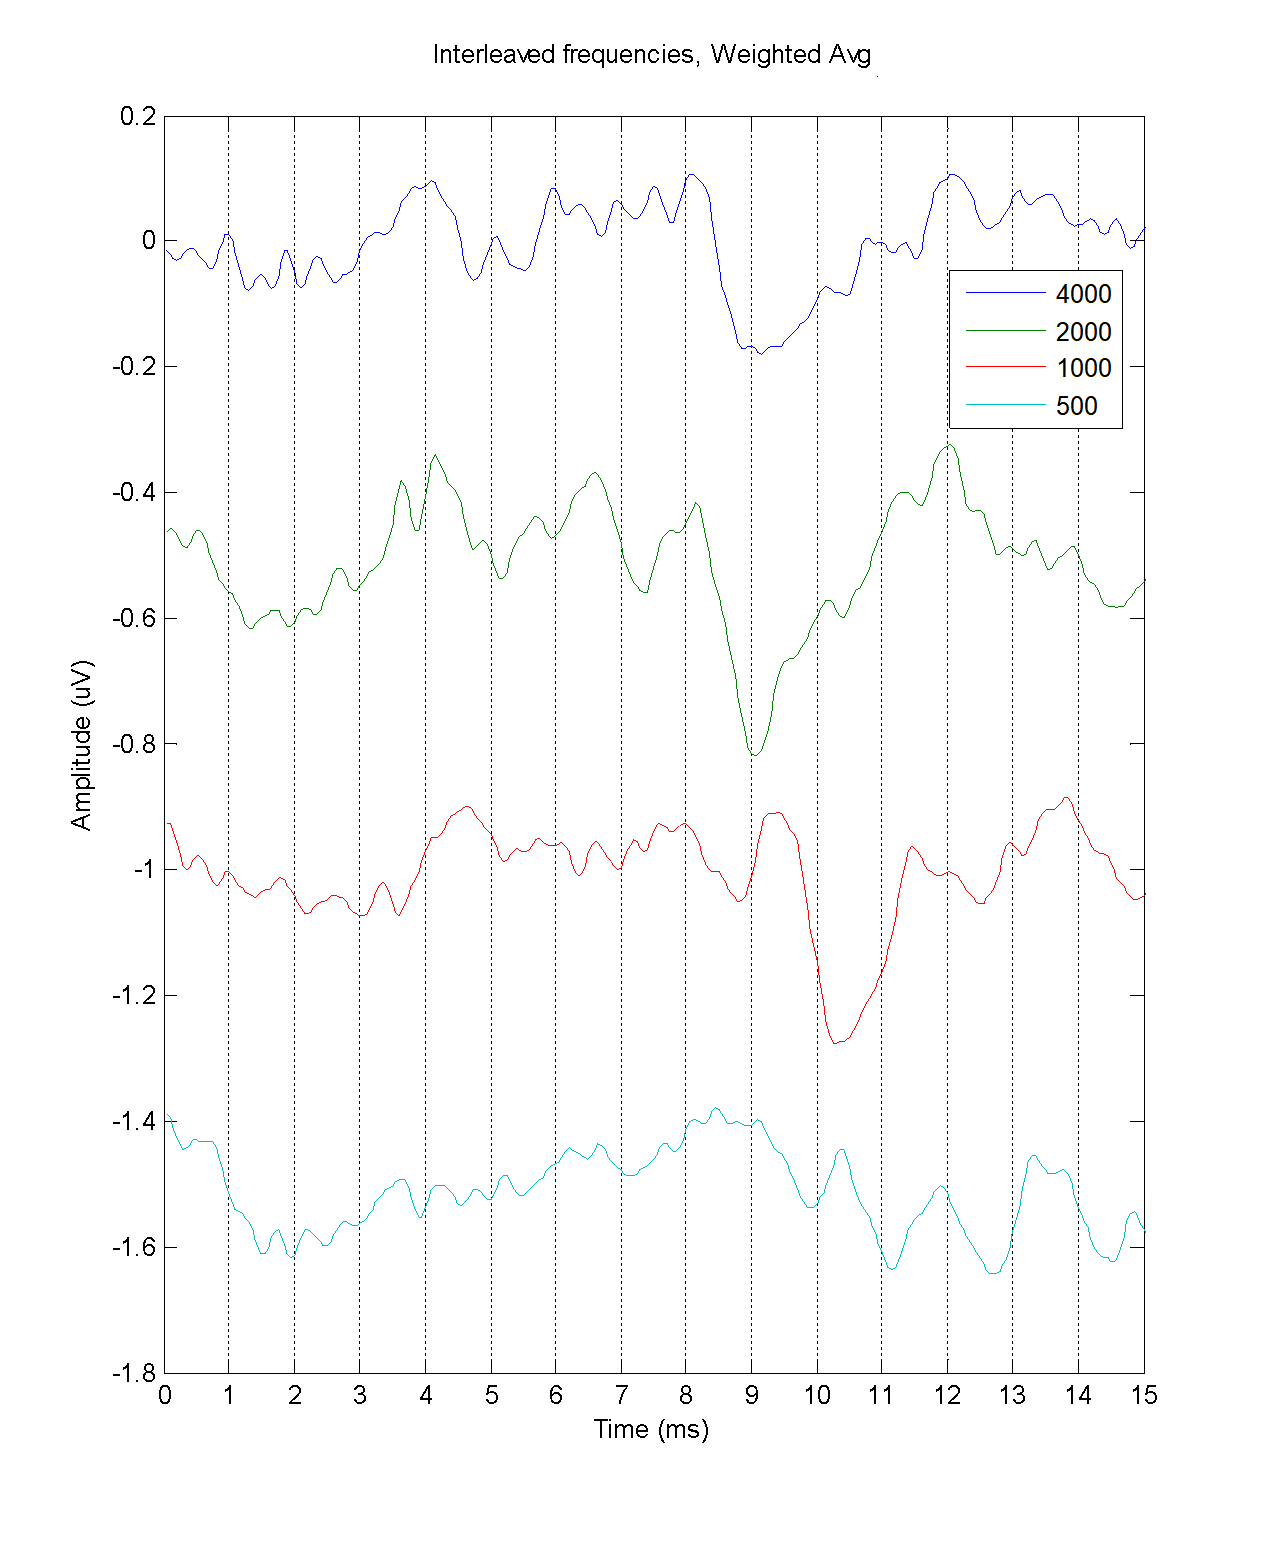
\includegraphics[width=\textwidth]{images/Interleaved75dbGHINOMA-2.png}
    \end{minipage}
    
    \vspace{0.2cm}
    
    \begin{minipage}{0.48\textwidth}
        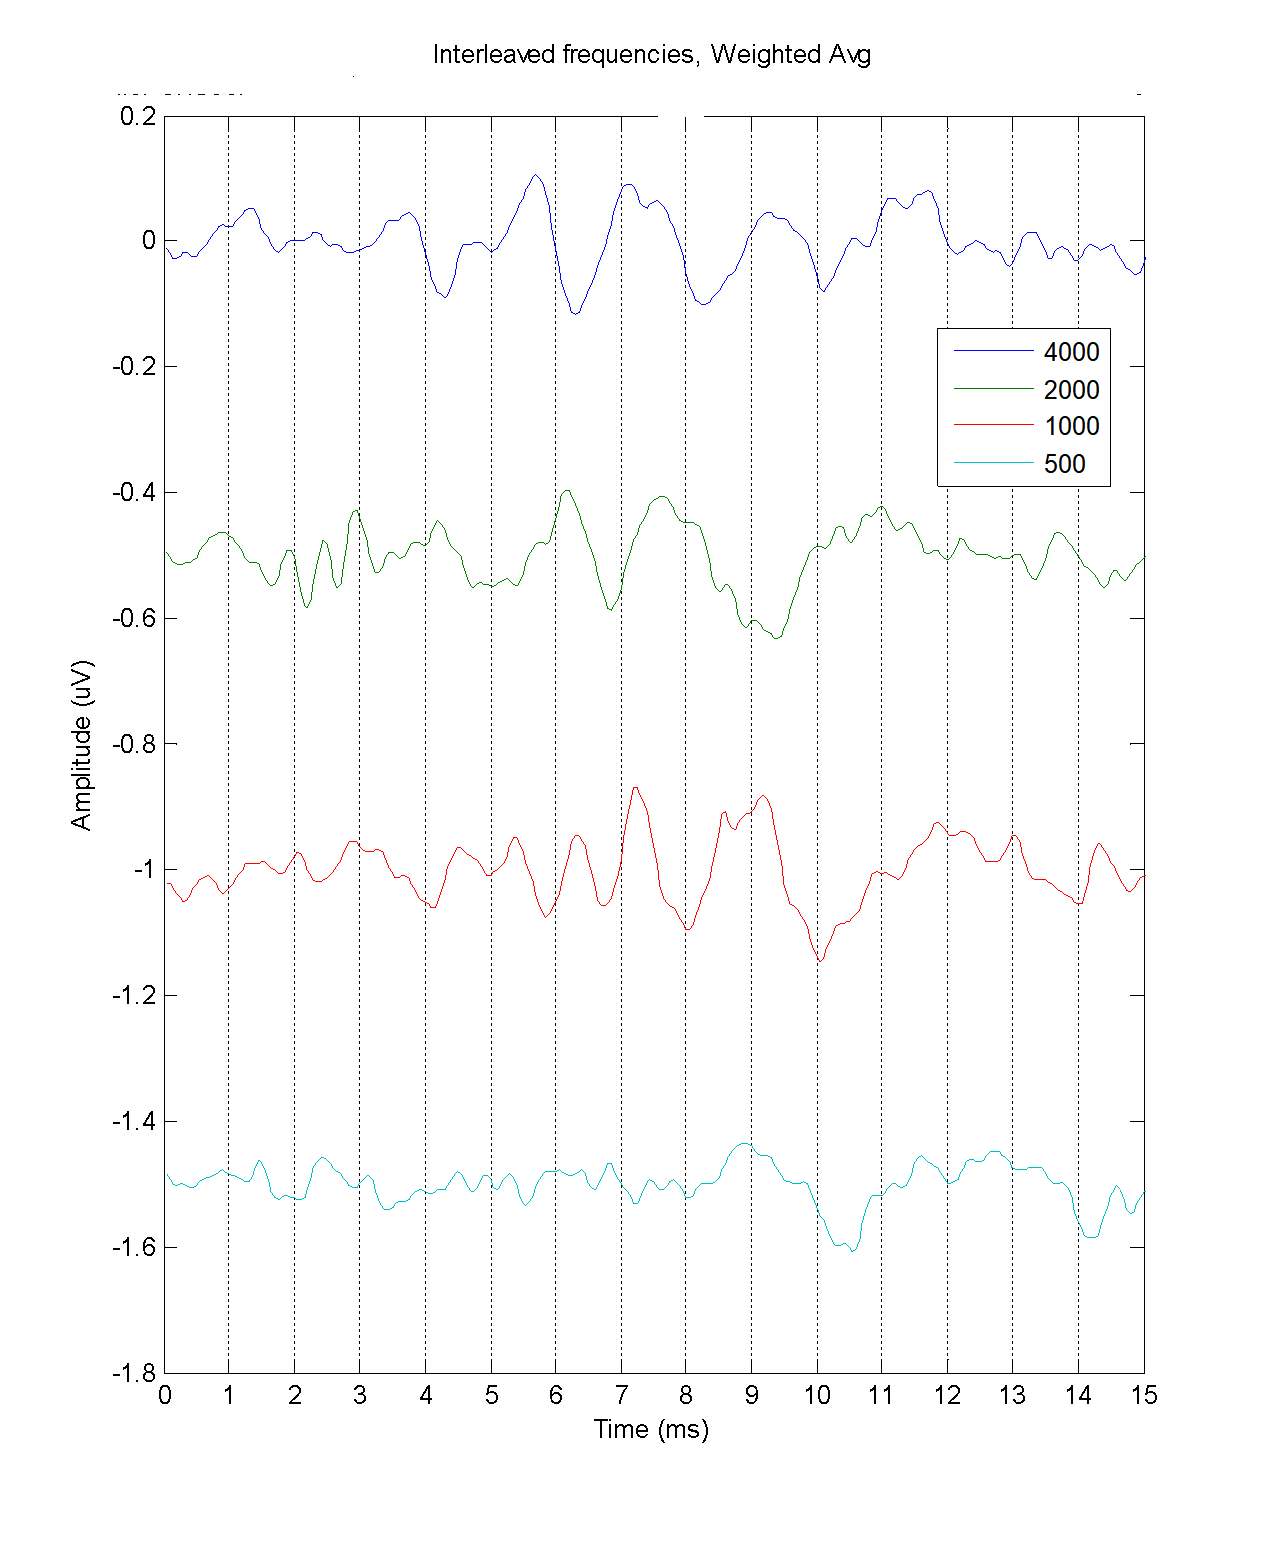
\includegraphics[width=\textwidth]{images/Interleaved75dbGHINOMA-3.png}
    \end{minipage}
    \hfill
    \begin{minipage}{0.48\textwidth}
        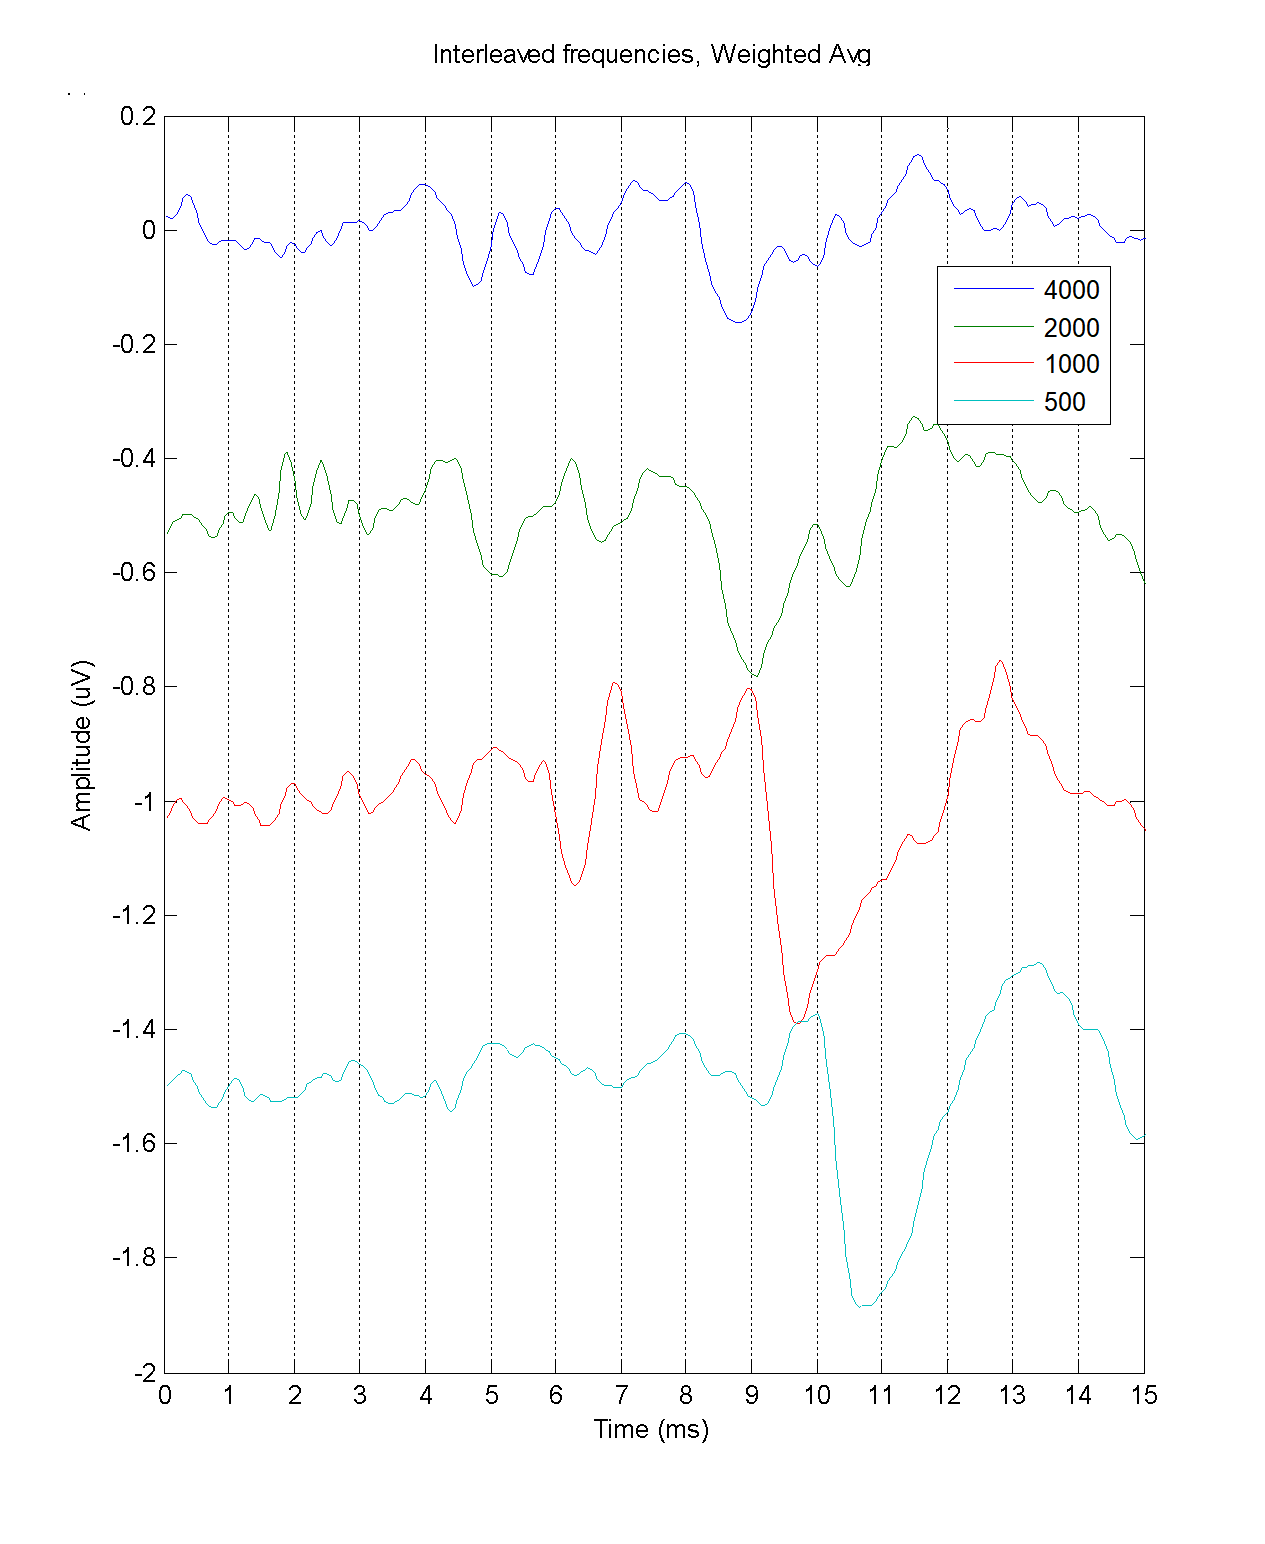
\includegraphics[width=\textwidth]{images/Interleaved75dbGHINOMA-4.png}
    \end{minipage}
    \caption{交替Tone(4kHz、2kHz、1kHz、500Hz)ABR 波形}
    \label{fig:Interleaved75dbGHINOMA}
\end{figure}


\begin{figure}[H]
    \centering
    \begin{minipage}{0.48\textwidth}
        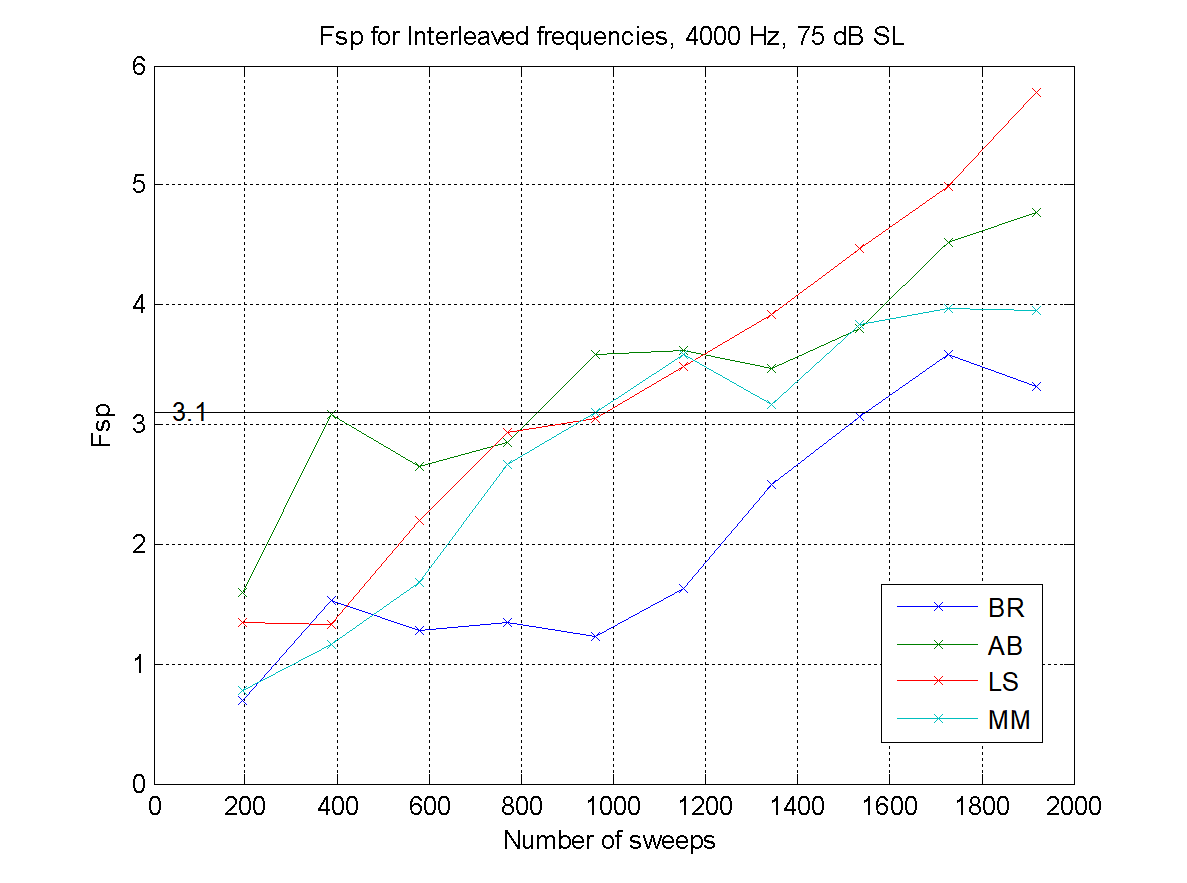
\includegraphics[width=\textwidth]{images/fspForInterleaved4000.png}
    \end{minipage}
    \hfill
    \begin{minipage}{0.48\textwidth}
        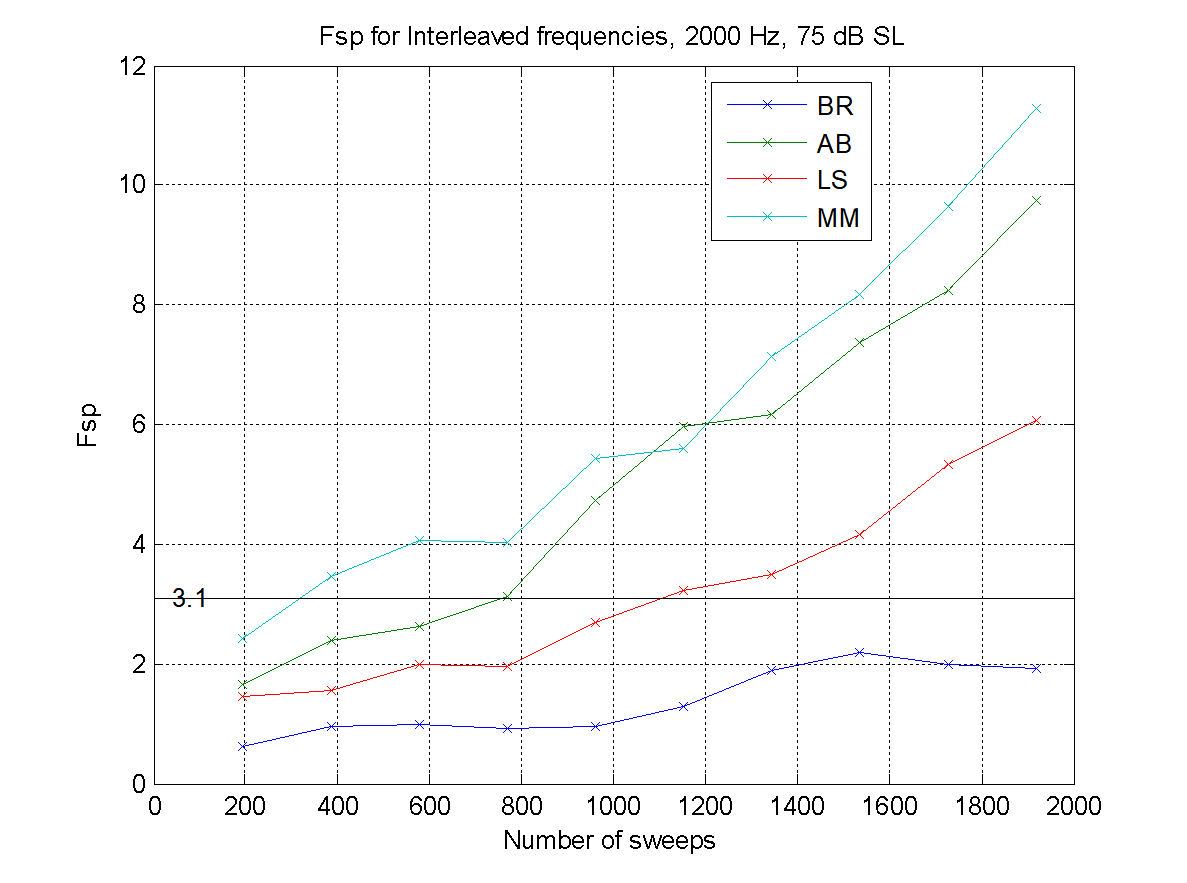
\includegraphics[width=\textwidth]{images/fspForInterleaved2000.png}
    \end{minipage}
    
    \vspace{0.2cm}
    
    \begin{minipage}{0.48\textwidth}
        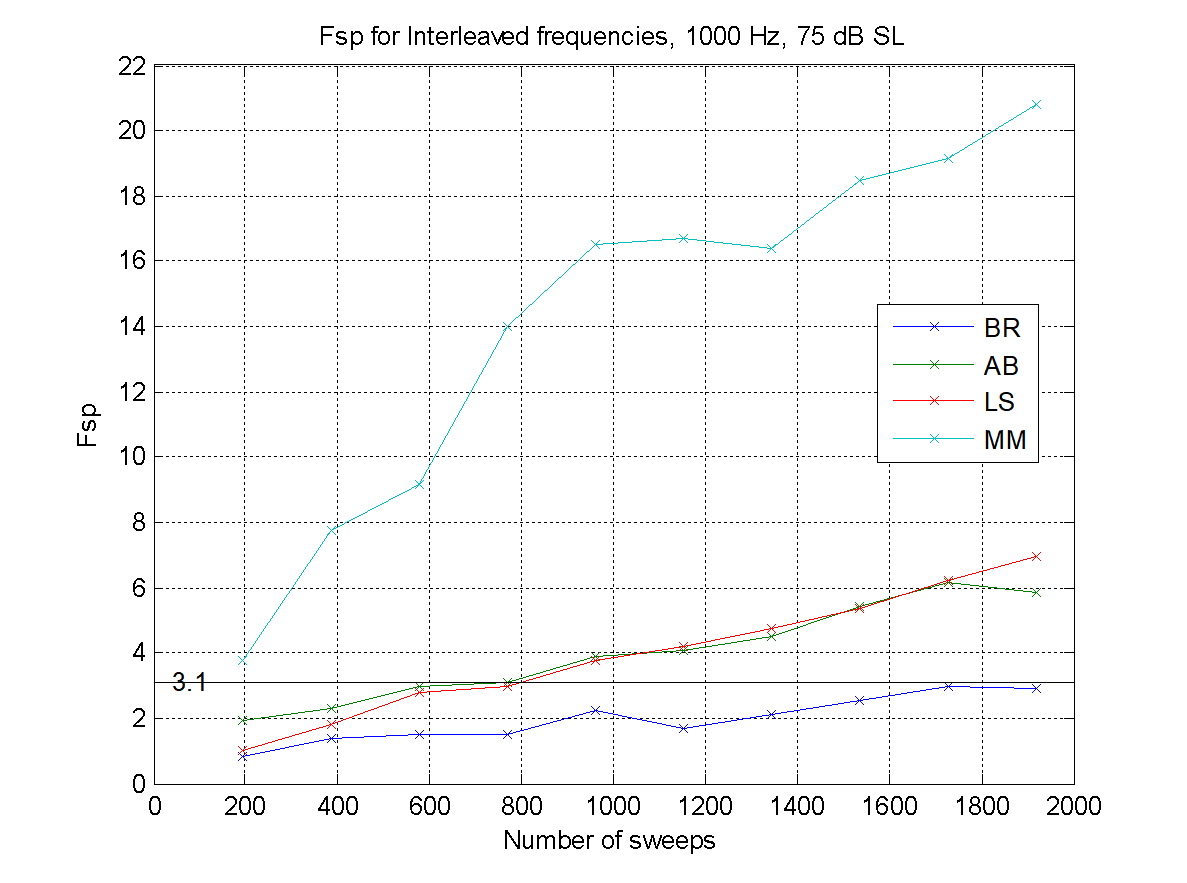
\includegraphics[width=\textwidth]{images/fspForInterleaved1000.png}
    \end{minipage}
    \hfill
    \begin{minipage}{0.48\textwidth}
        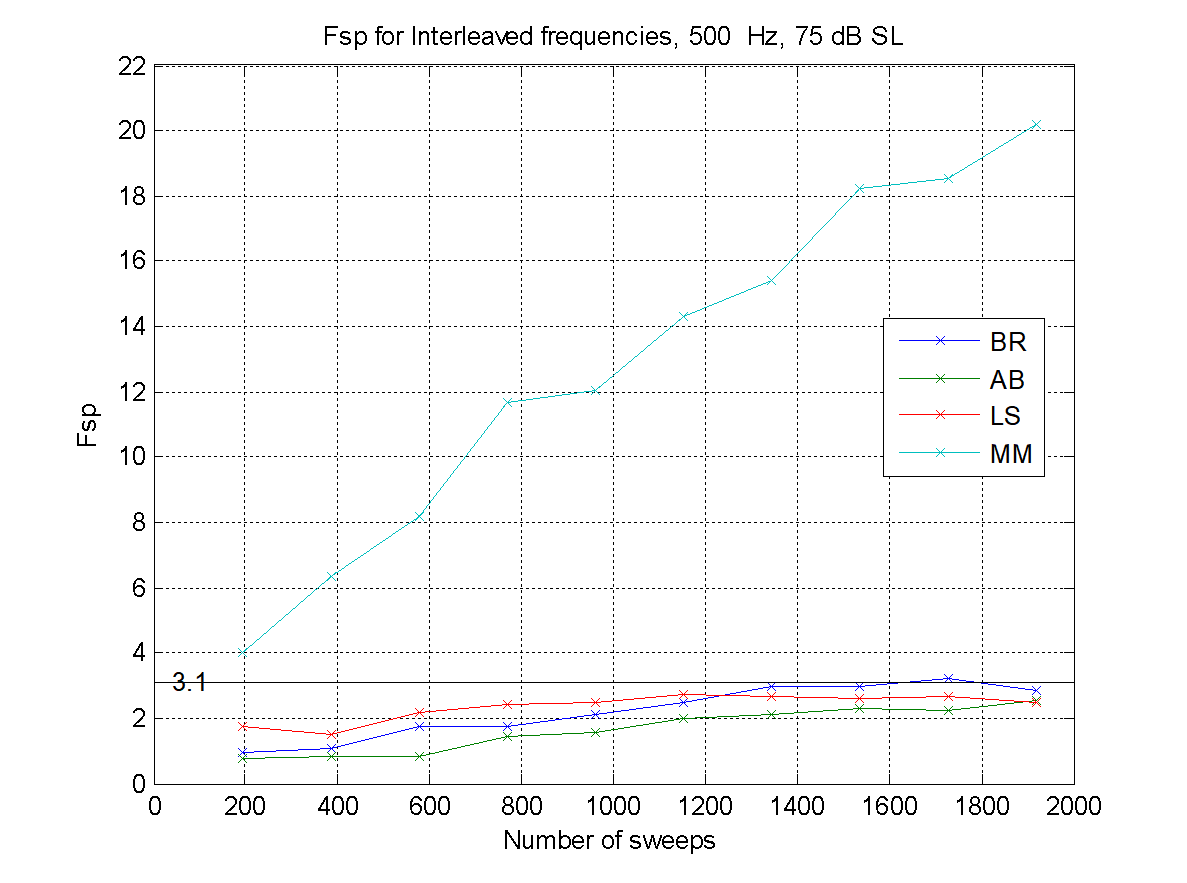
\includegraphics[width=\textwidth]{images/fspForInterleaved500.png}
    \end{minipage}
    \caption{交替Tone(4kHz、2kHz、1kHz、500Hz) F$_{sp}$ }
    \label{fig:Interleaved75dbGHINOMA}
\end{figure}

\paragraph*{带高通噪声掩蔽的交错频率刺激}
采用GHINOMA高通噪声掩蔽的交错频率刺激序列中的Tone刺激,与20 Hz呈现速率的单频刺激存在以下关键差异:
所有频率的Tone短声持续时间统一约为3 ms;采用高斯窗(Gaussian window)进行时域加窗处理
;
无噪声掩蔽条件下的刺激序列统一采用65 dB。

在交错频率刺激序列中,Chirp刺激与Tone刺激的F{$_sp$}比值存在显著频率依赖性差异:

\begin{itemize}
\item \textbf{4000 Hz与1000 Hz}:Chirp刺激的F$_{sp}$比值显著更高($p<0.05$)
\item \textbf{其他测试频率}:未观察到统计学显著差异
\end{itemize}

\textbf{主要结论:}
在本研究有限样本量条件下:

\begin{itemize}
\item 可识别响应所需的平均测试时长未显著缩短
\item 波形形态学特征的可解释性降低
\end{itemize}

\subsubsection{基于MLS的ABR响应}
MLS采用高刺激率的伪随机序列,通过快速连续呈现刺激信号,并利用解卷积技术分离重叠的神经响应,旨在缩短测试时间。本部分主要比较了标准解卷积和ISI依赖性解卷积两种方法对ABR信号质量的影响,并评估了MLS与传统刺激方法的优劣。

\textbf{MLS技术的基本原理}
\begin{itemize}
\item \textbf{高刺激率设计}:本部分采用的MLS刺激率是250Hz,远高于传统的10-20Hz,通过伪随机间隔的刺激序列实现时间压缩。
\item \textbf{解卷积处理}:由于响应重叠,需要采用数学方法分离各刺激对应的ABR成分。
\end{itemize}
\paragraph{标准解卷积方法}
MLS响应首先采用标准解卷积技术进行处理。研究以250Hz的刺激率呈现6阶序列(每扫描32个脉冲),并在每个扫描区块后计算F$_{sp}$值。
不同受试者之间,以及 4000 Hz 和 500 Hz Tone之间,F$_{sp}$ 值超过阈值 3.1 所需的时间存在显著差异。此外,虽然原本预期 4000 Hz Tone会更容易被检测到,但实际上并非总是如此。
在数据采集 100 秒后,研究将 MLS 刺激(250 Hz 速率)所引起的反应与传统刺激速率(20 Hz)所引起的反应进行了比较。


\paragraph{刺激间隔依赖性解卷积技术}
采用改进型\textbf{刺激间隔依赖性(ISI-dependent)解卷积算法}对MLS诱发的ABR响应进行处理,
标准的 MLS 解卷积假设序列中每个刺激所引起的反应是相同的。然而,由于序列中的刺激并非等间隔排列,而在间隔较近的刺激中,ABR峰的潜伏期更长。为了解决这个问题,研究引入了一种经过改进的、基于 ISI(刺激间隔)的解卷积方法,以考虑由此产生的额外延迟。

以一个MLS为例,其参数为:

序列长度:63

脉冲数量:32

最小刺激间隔(ISI):4 毫秒

其中,不同组别的脉冲数量及对应延迟为:

1 组脉冲:间隔为最小 ISI(4 ms)的脉冲:16 个 附加延迟为 α$_{1}$ 个采样点

2 组脉冲: 间隔为 2 倍最小 ISI(8 ms)的脉冲:8 个 附加延迟为 α$_{2}$  个采样点

3 组脉冲: 间隔为 3 倍最小 ISI(12 ms)的脉冲:4 个 附加延迟为 α$_{3}$  个采样点

由于一半的脉冲间隔为最短(4 ms),因此首先确定 α$_{1}$ 的最优值。在解卷积过程中,将所有 ISI 为 4 ms 的脉冲延迟不同的采样数量(从 0 到 28 个采样点),并观察平均解卷积结果中的 Wave V-V’ 峰的形状与幅值,从而确定最合适的延迟参数。
使用基于ISI去卷积方法处理ABR波形时,其F$_{sp}$值相比标准去卷积方法更高,表明信噪比有所提升,尽管Wave V的幅度并未显著改善。然而,从某些受试者虚线波形来看,存在未能完全抵消的波峰,同时F$_{sp}$值在叠加次数增加时并未持续提高,说明该方法尚不理想,有待进一步优化。由于这些非抵消波峰来自与 α$_{1}$ 和 α$_{2}$ 参数设置时不同的受试者,说明在紧密刺激下产生的额外潜伏时间可能具有个体差异性。此外,已有研究指出刺激频率增加所引起的波形潜伏期变化还受到背景噪声水平的影响,因此 α$_{1}$ 和 α$_{2}$ 若采用固定值,可能无法适用于所有实验条件。

\subsubsection{自适应滤波的影响}
\paragraph*{维纳滤波方法}
\textbf{信号估计策略}

采用了三种不同的信号估计策略以提高ABR信号的识别准确性。
\begin{itemize}
\item 系统在累计完成2000次扫描后一次性对数据进行统一处理
\item 则在达到250次扫描后即启动实时处理
\item 基于受试者的ABR响应谱构建先验模板
\end{itemize}
\textbf*{频谱分析方法}
每个刺激后的15\,ms时段信号进行512点快速傅里叶变换(FFT)分析,以提取ABR响应的频谱特征。在频谱分析前,信号经过100–3000\,Hz的带通滤波预处理,以去除低频漂移和高频噪声。此前验证了100–1000\,Hz的窄带设置,但结果显示其在信噪比提升方面无显著改进。滤波器设计方面,采用128阶有限冲激响应(FIR)滤波器。

\subsection*{对比方法与评估指标}
为了全面评估 ABR 响应的有效性与质量,本文选取了四项关键指标进行分析。首先,Wave V 振幅是指 Wave V 峰值与后续谷值之间的电压差,以微伏(μV)为单位,数值越大代表神经同步反应越强,信号识别性越好。其次,F$_{sp}$ 比值用于衡量信号整体方差与单点噪声方差之间的关系,当比值大于 3.1 时,通常视为存在显著的神经反应,是信噪比可靠性的判断依据之一。第三项指标是潜伏期,即从刺激开始到 Wave V 峰值出现之间的时间间隔,单位为毫秒(ms),正常范围在 6.5 至 7.5 毫秒之间,用于反映神经传导速度及完整性。最后,Hotelling's T² 统计量是一种多变量统计方法,通过分析多个时间点的波形变化,来评估 ABR 波形是否显著区别于背景噪声,当 p 值小于 0.05 时表示检测结果具有统计学显著性。综合这些指标可多角度判断神经反应的存在与特征,有助于提高 ABR 分析的敏感性与可靠性。

\subsection*{性能比较}
\paragraph*{定量结果}
\textbf{75dB数据}

\begin{table}[H]
\centering
\caption{不同刺激类型在75dB SL强度下的ABR参数比较}
\label{tab:75dbstimulus_comparisonParameter}
\begin{tabular}{lcccc}
\toprule
\textbf{刺激类型} & \textbf{Wave V振幅(\si{\micro V})} & \textbf{F$_{sp}$比值} & \textbf{潜伏期(ms)} & \textbf{Hotelling's T²值} \\
\midrule
Click(疏波) & $0.37 \pm 0.03$ & 4.1 & $6.4 \pm 0.3$ & $<0.001$ \\
Click(密波) & $0.35 \pm 0.04$ & 3.8 & $6.6 \pm 0.4$ & 0.002 \\
宽带 Chirp & $0.27 \pm 0.05$ & 3.0 & $6.2 \pm 0.4$ & 0.003 \\
\SI{4}{kHz} 窄带 Chirp & $0.16 \pm 0.02$ & 4.2 & $7.3 \pm 0.4$ & $<0.001$ \\
\SI{500}{Hz} Tone Burst & $0.12 \pm 0.03$ & 2.8 & $9.5 \pm 0.5$ & 0.008 \\
MLS Click & $0.30 \pm 0.04$ & 3.8 & $6.7 \pm 0.5$ & $<0.001$ \\
\bottomrule
\end{tabular}
\end{table}

\begin{table}[H]
\centering
\caption{不同刺激类型在40dB SL强度下的ABR参数比较}
\label{tab:40dbstimulus_comparisonParameter}
\begin{tabular}{lcccc}
\toprule
\textbf{刺激类型} & \textbf{Wave V振幅(\si{\micro V})} & \textbf{F$_{sp}$比值} & \textbf{潜伏期(ms)} & \textbf{Hotelling's T²} \\
\midrule
Click(疏波) & $0.23 \pm 0.05$ & 2.1 & $8.41\pm 0.3$ & 0.003 \\
Click(密波) & $0.18 \pm 0.04$ & 1.8 & $8.6 \pm 0.4$ & 0.010 \\
宽带 Chirp & $0.46 \pm 0.08$ & \textbf{3.8} & $8.2 \pm 0.4$ & $<0.001$ \\
\SI{4}{kHz} 窄带 Chirp & $0.11 \pm 0.03$ & 2.3 & $9.1 \pm 0.5$ & 0.012 \\
\SI{500}{Hz} Tone Burst & $0.15 \pm 0.03$ & 2.6 & $10.8 \pm 0.6^{\dagger\dagger}$ & 0.020 \\
MLS Click & $0.25 \pm 0.06$ & \textbf{3.5} & $8.8 \pm 0.7$ & 0.002 \\
\bottomrule
\end{tabular}
\end{table}

\noindent \footnotesize 注:\\
1.数据表示为$\text{均值} \pm \text{标准差}$\\
2.F$_{sp}$比值阈值设为3.1(99\%置信水平)\\
3.采样率=\SI{20}{kHz},带通滤波={100 - 3000}{Hz}
\normalsize 

\textbf{关键差异对比}
\begin{table}[H]
\centering
\caption{不同声压级下ABR特征对比}
\begin{tabular}{|l|c|c|}
\hline
\textbf{特征} & \textbf{75 dB SL} & \textbf{40 dB SL} \\
\hline
最佳刺激 & Click(Wave 0.37μV) & Broadband Chirp(Wave 0.46μV) \\
\hline
潜伏期变化 & 基准值(Click 6.4ms) & 普遍延长2.0-2.5ms \\
\hline
F$_{sp}$阈值 & 普遍>3.5 & 普遍降低0.5-1.0个单位 \\
\hline
MLS效率 & 检测时间60秒(↓40\%) & 保持高效(60秒) \\
\hline
低频响应 & 500Hz Tone Burst 0.12μV & 需交替极性提升至0.15μV \\
\hline
\end{tabular}
\end{table}

在不同声压级条件下,ABR 的特征表现出显著差异。高声压(75 dB SL)下,Click 刺激具有更高的波幅(0.37μV)和较短的潜伏期(6.4ms),F$_{sp}$ 指标普遍高于 3.5,MLS 检测效率提升了约 40\%。低声压(40 dB SL)下,Broadband Chirp 更具优势,产生更强的响应(0.46μV),但潜伏期普遍延长 2.0 至 2.5ms,F$_{sp}$ 阈值有所降低。为了提升低频响应,在 500Hz 处需采用交替极性以获得更佳波幅(由 0.12μV 提升至 0.15μV)。
\subsection*{主观实验}
本实验旨在通过主观评估,验证不同刺激类型在ABR测试中对Wave V响应的影响是否与报告中的客观数据一致,重点考察的指标包括Wave V振幅、F$_{sp}$比值、潜伏期和Hotelling's T² 值。实验共招募5名听力正常的成年志愿者,其Tone听力阈值均在250至8000 Hz范围内不超过20 dB HL,且无耳科病史。使用Neuroscan系统配合插入式耳机进行刺激播放,ABR信号通过四通道电极(Cz-Inion、Cz-A1、T1-T2、T1-A1)记录,采样率为20 kHz。刺激设计根据报告推荐,涵盖宽带Click、宽带及窄带 Chirp、交替极性Tone以及 MLS ,并在75 dB和40 dB SL两个强度水平下进行。每位参与者随机接受所有刺激类型的ABR测试,每种条件记录2000至3000次扫描以确保信噪比。主观评分由听力师根据匿名呈现的ABR波形图对Wave V的清晰度、潜伏时间感知(快/慢)以及背景噪声干扰程度进行打分,满分5分。同时记录实际的Wave V振幅、F$_{sp}$比值、潜伏期和Hotelling's T²值。初步预期宽带Chirp或MLS在40 dB下的清晰度评分将显著优于 Click,匹配报告中更高的F$_{sp}$值;而在4 kHz和500 Hz条件下,窄带Chirp与交替极性Tone也可能获得更高主观评分,与其在报告中的客观优势一致。尽管样本量有限,主观评分可能受解读偏差影响,但本实验提供了一个将客观ABR性能与实际临床感知相结合的验证框架,对刺激类型的优化具有参考意义

\subsection*{分析与讨论}
\subsubsection{不同刺激类型对Wave V振幅的影响}
实验结果显示,宽带 Chirp 在40 dB SL的低刺激强度下显著提高了Wave V振幅,这与报告中提到的“Chirp刺激在低强度下能增强神经同步性”的结论一致。然而,在75 dB SL的高强度下,Click的表现优于Chirp,可能由于高强度下低频率能量导致基底膜不同区域的响应重叠,从而降低同步性。
对于4 kHz窄带刺激,75 dB SL下常规Tone结合自适应滤波的Wave V振幅最高,而40 dB SL下窄带Chirp表现更优。这表明,Chirp刺激在低强度、高频(如4 kHz)条件下能有效补偿耳蜗基底膜的频率依赖性延迟。
500 Hz交替极性Tone在75 dB SL和40 dB SL下均表现出较高的Wave V振幅,尤其是与单极性Tone相比。这可能是由于交替极性减少了刺激伪迹(如肌电干扰),从而提高了 SNR 。然而,500 Hz的响应整体较4 kHz更不稳定,可能与低频刺激的耳蜗传播时间较长有关。

\subsubsection{F$_{sp}$比值与信号检测效率}
F$_{sp}$比值反映了信号(ABR波形)与噪声(背景EEG)的方差比,较高的F$_{sp}$值通常意味着更可靠的检测。实验发现:
宽带刺激:40 dB SL下,Chirp和MLS的F$_{sp}$值显著高于短声,支持报告中“MLS和Chirp在低强度下更具优势”的结论。
4 kHzTone:75 dB SL下,自适应滤波显著提高了F$_{sp}$值,说明该方法能有效抑制噪声(如50 Hz工频干扰)。
500 Hz交替极性Tone:F$_{sp}$值明显优于单极性Tone,进一步验证了交替极性在低频ABR检测中的重要性。
然而,部分受试者在40 dB SL下的F$_{sp}$值仍低于3.1(新生儿筛查的常用阈值),表明在极低刺激强度下,可能需要更长的平均时间或更优化的刺激参数(如调整Chirp的频谱特性)。

\subsubsection{潜伏期变化与刺激类型的关系}
宽带刺激:Chirp刺激的Wave V潜伏期比短声长约10 ms,这与Chirp的时频调制特性一致(Dau et al., 2000)。
4 kHzTone:常规Tone的潜伏期(~7.2 ms)与文献一致,而MLS序列的潜伏期略有增加,可能与高刺激率导致的神经适应有关。
500 HzTone:潜伏期最长(~10.8 ms),符合低频刺激在耳蜗中的传播延迟特性。
值得注意的是,部分受试者的潜伏期比文献报道的略长(如短声刺激下7.2 ms vs. 标准6.4 ms),可能与Neuroscan系统的触发延迟有关(报告中提到可能存在0.8 ms的延迟)
\subsubsection{Hotelling's T²与 F$_{sp}$ 的比较}
Hotelling's T² 和 F$_{sp}$ 在大多数情况下表现一致,但Hotelling's T²在4 kHz刺激下略优于F$_{sp}$,可能因为Hotelling's T²对波形的时间结构更敏感(如Wave V的斜率变化)。然而,F$_{sp}$的计算更简单,适合临床快速筛查。
实验还发现,对ABR的导数(derivative)应用Hotelling's T²时,检测效率略有提升,尤其是早期时间窗口(如Wave III-V区间),这与“Wave V的陡峭负斜率是重要检测特征”的假设一致。


\subsubsection{最佳刺激方案与信号处理总结}
\begin{table}[H]
\centering
\caption{最佳刺激方案与信号处理总结}
\label{tab:beststimulusSignalProcessing}
\begin{tabular}{|l|p{5.5cm}|p{5.5cm}|}
\hline
\textbf{刺激类型} & \textbf{75 dB SL 设置} & \textbf{40 dB SL 设置} \\
\hline
宽带刺激 & 
Click结合(Wiener滤波) &
宽带Chirp结合自适应滤波,或采用MLS\\
\hline
4 kHz窄带刺激 & 
Tone结合自适应滤波 &
窄带Chirp\\
\hline
500 Hz窄带刺激& 
交替极性Tone结合自适应滤波 &
交替极性Tone,或采用MLS \\
\hline
\multicolumn{3}{|l|}{\textbf{信号处理方法:} 自适应滤波 / Wiener滤波} \\
\hline
\end{tabular}
\end{table}
